
This chapter presents a communication interface for different simulator domains. These will be integrated into Gem5 and SystemC, representing 
a new contribution since no existing solutions are present in the current state of the art. Further, it was selected a 
case study, which serves as a stimulus for system design and demonstrates 
the practical application of the developed work. The chosen case study focuses on the \gls{crc} peripheral, developed on SystemC which interfaces 
as an external peripheral on gem5's board. 

To close the chapter, par-gem5 with both static and dynamic versions will be tested with the developed interface. 
The obtained results will be presented and compared to the ones conducted in sequential mode in order to have an evaluation reference. 
Concerning the results, an approach will be selected, being it the preferred to address other situations. 

\section{Framework Proposal}

As previously mentioned on \autoref{cap:SoA}, co-simulation involves the integration of multiple simulation tools from different
domains. Therefore, it is required to develop a system that could execute and communicate among them. This system must adhere to three key 
aspects to ensure a well-functioning environment. The first one is data integrity. Both tools must respect the defined data exchange standards 
otherwise, data may become corrupted, creating a failure in the simulation ecosystem. The second aspect is data exchange. A proper delineation of the 
interface where data will flow is important as well. Missing this may result in faulty communication channels. The last one is the synchronization 
between both simulators, since improper synchronization may lead to causality errors.

Regarding these concerns, it was proposed the framework presented in the following picture. It will be composed of three interfaces: Gem5, SystemC, 
and remote port. Gem5 and SystemC are two simulators already introduced in the state-of-the-art chapter however, other simulators could be used. 
The remote port interface was defined to allow communication between the tools.

\begin{figure}[H]
	\centering
 	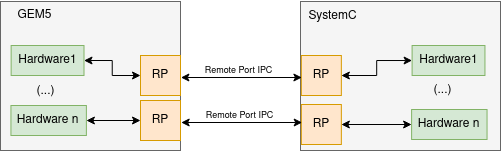
\includegraphics[width=0.8\linewidth]{Images/CoSimDesignSimplified.png}
 	\caption{High-level proposal design of the framework}
	 \label{fig_CoSimDesignSimplified}
\end{figure}

It exchanges data utilizing the TCP/IP \gls{ipc} protocol, due to its application independence and its versatility for various applications 
and purposes. Furthermore, this type of connection can be used remotely, by having multiple simulators running on different machines.  
As shown in the previous figure, each hardware device will have a unique connection to avoid concurrency problems. Furthermore, each simulator 
will perform distinct tasks on the remote port interface, necessitating unique definitions for each.

\subsection{Remote Port Interface} 
\label{subsec::TLMwrapper}

As already mentioned, the remote port interface will establish the communication between Gem5 and SystemC.
Although they are two simulators that use C++, they cannot communicate directly with each other. Gem5 is unable to 
interpret the \gls{tlm} commands, just as SystemC doesn't understand gem5 packages. For these reasons,
this interface will require a wrapper to enable communication between the two platforms. 
The wrapper will be available in both tools, and every transaction must be created regarding its definition otherwise, 
data integrity may be compromised. 

\begin{figure}[H]
	\centering
 	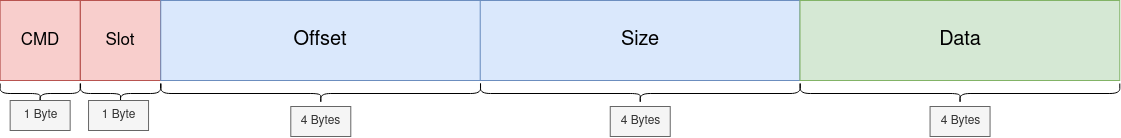
\includegraphics[width=0.8\linewidth]{Images/TLM_Wrapper_Payload.png} 
 	\caption{TLM wrapper payload definition}
	% \label{fig_TLM_Wrapper_Payload}
\end{figure}


The main part of the wrapper is the payload definition. It provides a unique definition to transport data and perform operations, 
keeps the transactions easy to understand, and improves efficiency. For this case, its definition can be found in the prior image. 
It can be divided into three sections: the remote port header, marked with red; the preamble data, marked with blue; and the data, marked with green. 
It is important to mention that the remote port's design was done regarding a 32-bit machine, reason why the data address, data size, and data value 
parameters have a four-byte length.

Every operation must begin with the payload header, which is composed of a command and a slot. The command indicates the operation to execute, and
its list can be found on \autoref{tab_TLMwrapperCMD}. The slot is used as an ID to decode where the operation should be done. 
As shown in \autoref{fig_CoSimDesignSimplified}, each hardware module connected to a remote port has a number associated, which can be indexed by 
the slot. Preamble data comes after the header, and it indicates the location where the execution will take place in the selected hardware. 
The data address or offset points to the desired hardware address and the data size specifies the action range. The data is required in 
the case of writing, since the new value must be known. 


\begin{table}[h!]
	\centering
	\begin{tabular}{llll}
	\cline{1-3}
	\multicolumn{1}{|l|}{\cellcolor[HTML]{C0C0C0}{\color[HTML]{000000} Bits}} & \multicolumn{1}{l|}{\cellcolor[HTML]{C0C0C0}{\color[HTML]{000000} Command}} & \multicolumn{1}{l|}{\cellcolor[HTML]{C0C0C0}{\color[HTML]{000000} Required Sections}} \\ \cline{1-3}
	\multicolumn{1}{|l|}{00} & \multicolumn{1}{l|}{TLM\_INIT} & \multicolumn{1}{l|}{Header} \\ \cline{1-3}
	\multicolumn{1}{|l|}{01} & \multicolumn{1}{l|}{TLM\_CLOSE} & \multicolumn{1}{l|}{Header} \\ \cline{1-3}
	\multicolumn{1}{|l|}{10} & \multicolumn{1}{l|}{TLM\_READ} & \multicolumn{1}{l|}{Header | Preamble data} \\ \cline{1-3}
	\multicolumn{1}{|l|}{11} & \multicolumn{1}{l|}{TLM\_WRITE} & \multicolumn{1}{l|}{Header | Preamble data | Data} \\ \cline{1-3}
	 &  & 
	\end{tabular}%
	\caption{TLM wrapper commands}
	\label{tab_TLMwrapperCMD}
\end{table}

Every transaction is followed up with a response, \textit{TLM\_ACK} (0) for success, or \textit{TLM\_NACK} (1) for error, and the operation 
latency, which is required to maintain the synchronization between the simulators. 

The next figures demonstrate how the wrapper is implemented in both tools. First of all, it is mandatory to initialize the remote port interface.
To accomplish that, Gem5 must start with the \textit{TLM\_INIT}, and wait for a positive response from SystemC. Only after that, the remote port 
is available, and write and read operations can proceed. Closing the remote port follows a similar path. Gem5 must call the \textit{TLM\_CLOSE}, and 
wait for \textit{TLM\_ACK} from SystemC. The wrapper always verifies if the remote port is available for transactions, and in case of an error, it 
returns a permission-denied notification. 

In read-and-write operations, the device's availability is crucial to maintain the tools synchronized. Picture a scenario where Gem5 sends 
two write requests and each write operation takes four clock cycles. When Gem5 executes the first request, SystemC will return a latency of 
four clock cycles. Consequently, whether another attempt is made in the next clock cycle, the device will still be processing the first one, 
resulting in a synchronization conflict. For this reason, if the device is unavailable, the busy notification is returned, indicating a need to 
retry the operation later.

In SystemC, while \textit{TLM\_INIT} and \textit{TLM\_CLOSE} are identical to Gem5 ones in the way of operating, \textit{TLM\_READ} and 
\textit{TLM\_WRITE} have some differences. First of all, instead of sending the transaction, it receives it and verifies if the received slot is accessible.
After that, it executes the respective \gls{tlm} operation, which can result in an error, for example, 
the offset crossed the device's boundaries, or in a successful process, returning to Gem5 the respective data. Further in this chapter, these 
operations will be explained in detail. 


\begin{figure}[H]
	\centering
 	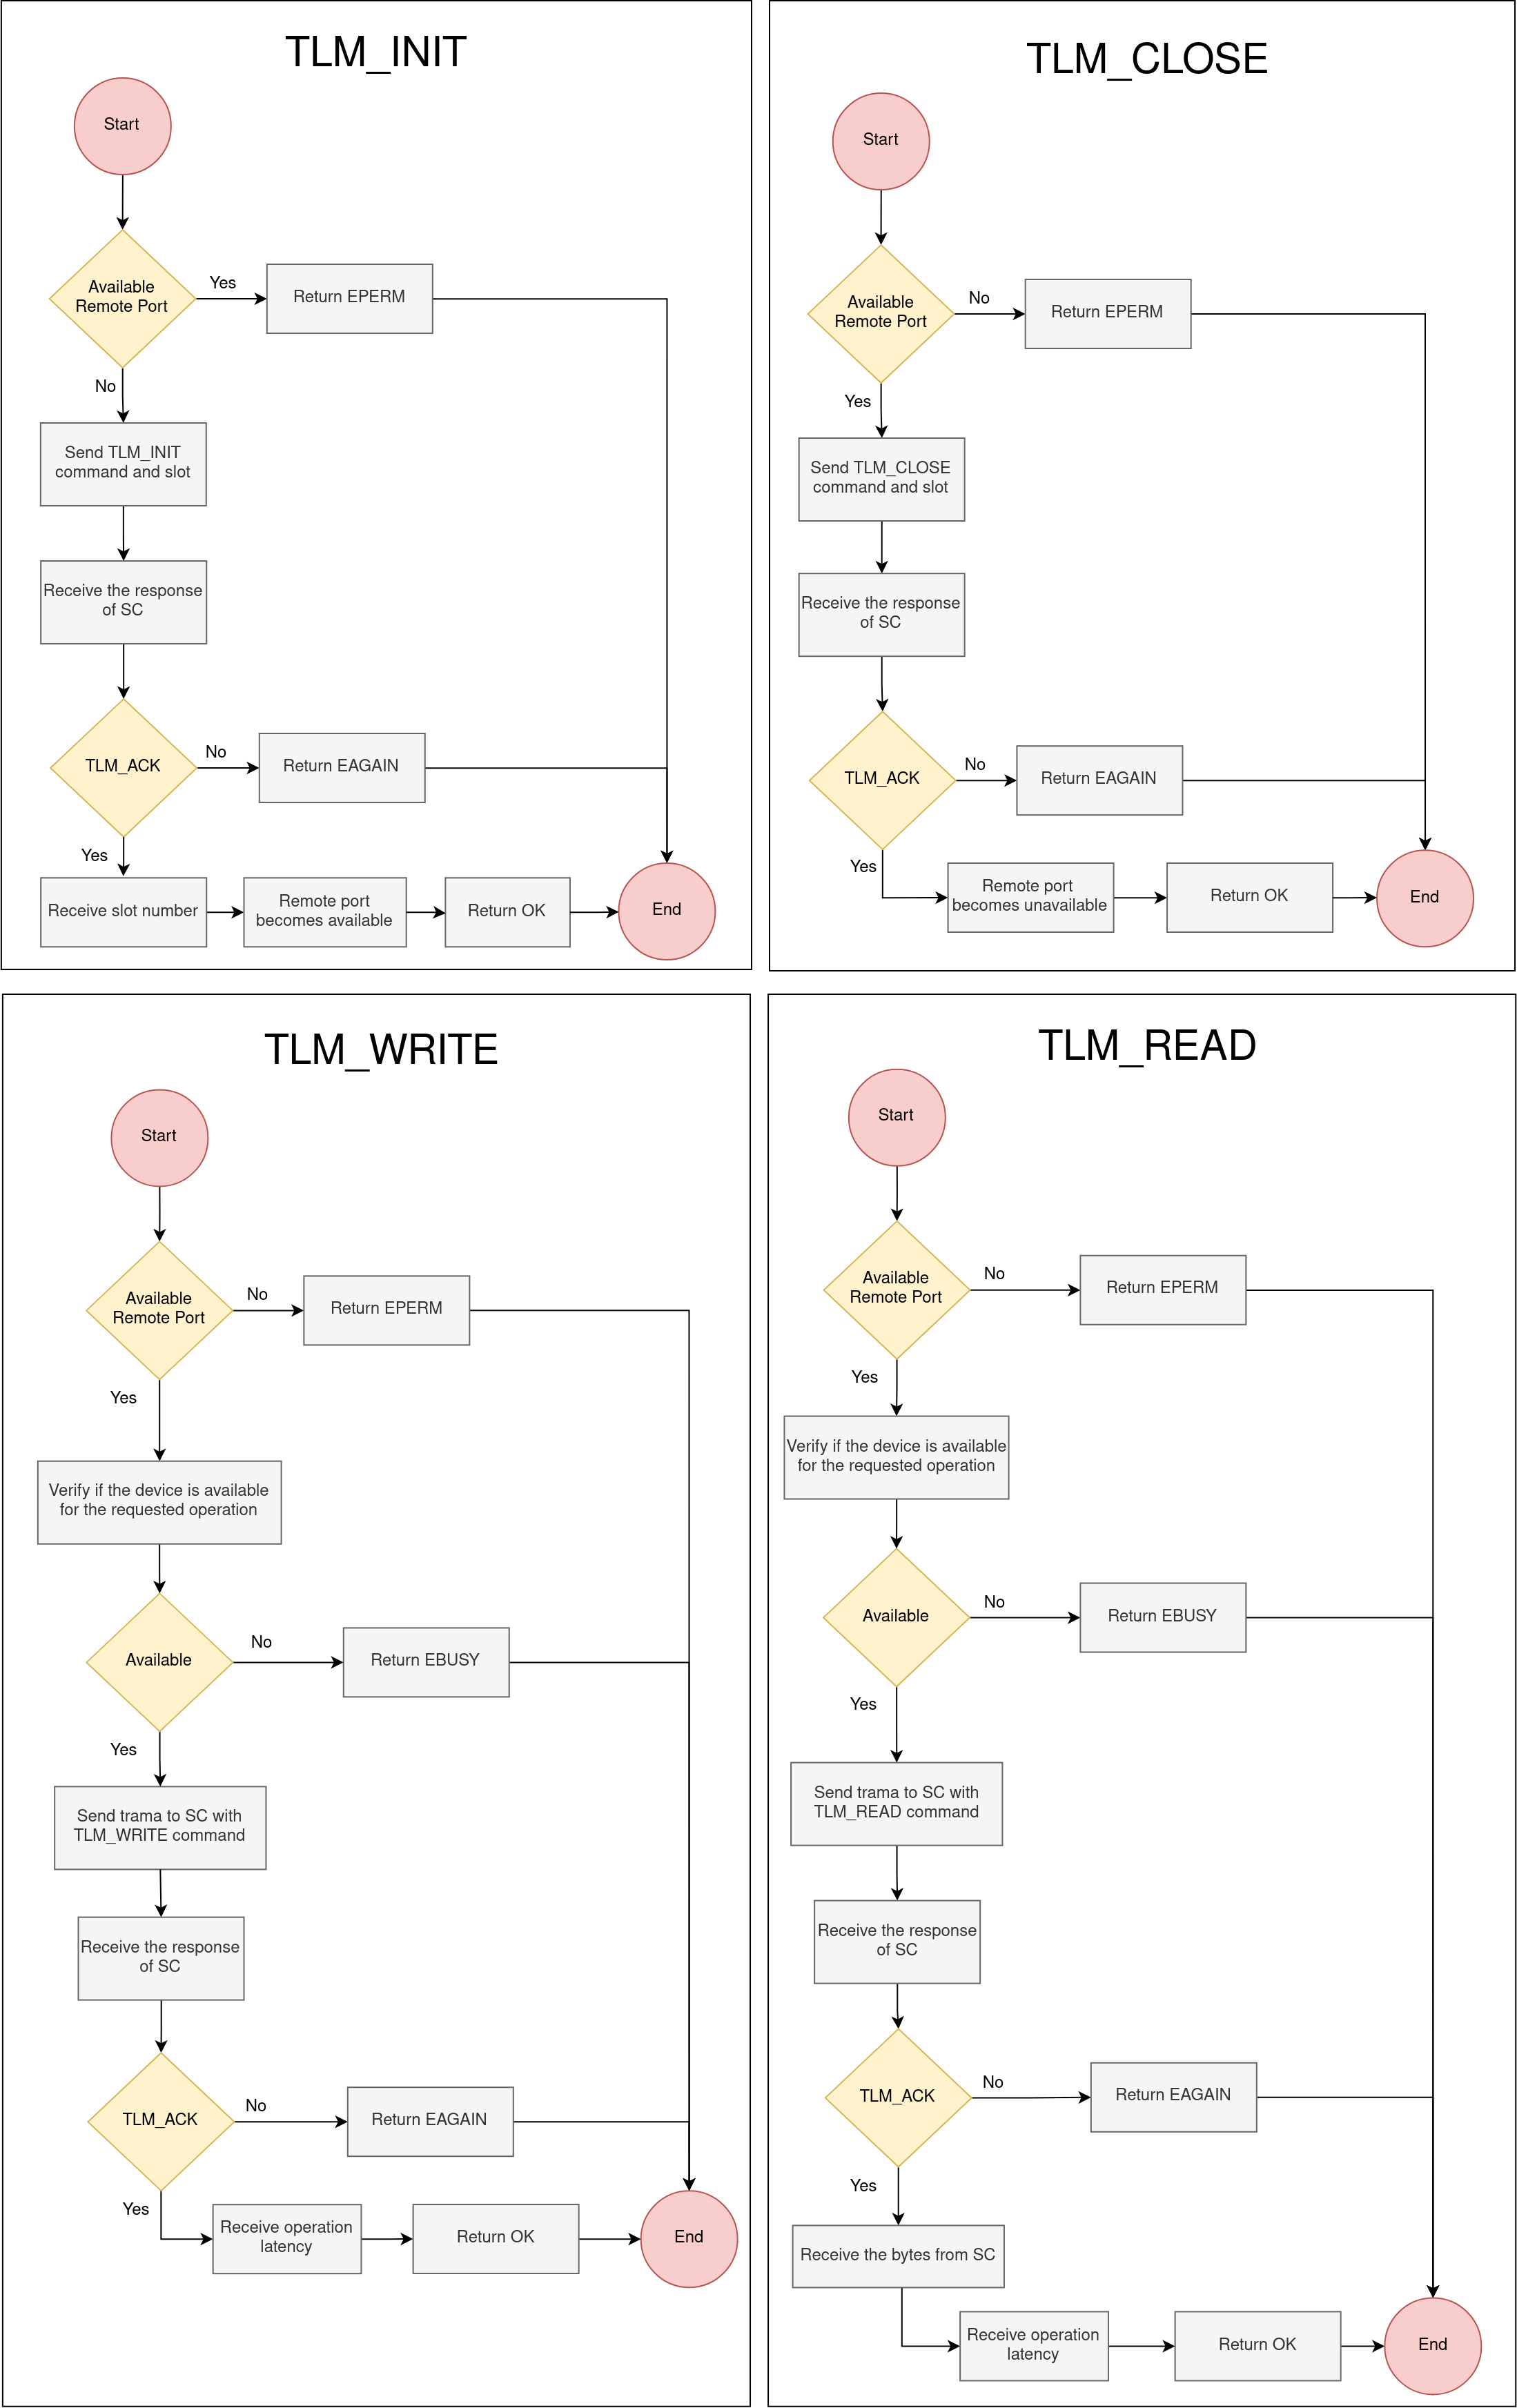
\includegraphics[width=0.8\linewidth]{Images/TLMWrapper_Gem5.png} 
 	\caption{TLM wrapper in Gem5}
	% \label{fig_TLM_Wrapper_Payload}
\end{figure}

\begin{figure}[H]
	\centering
 	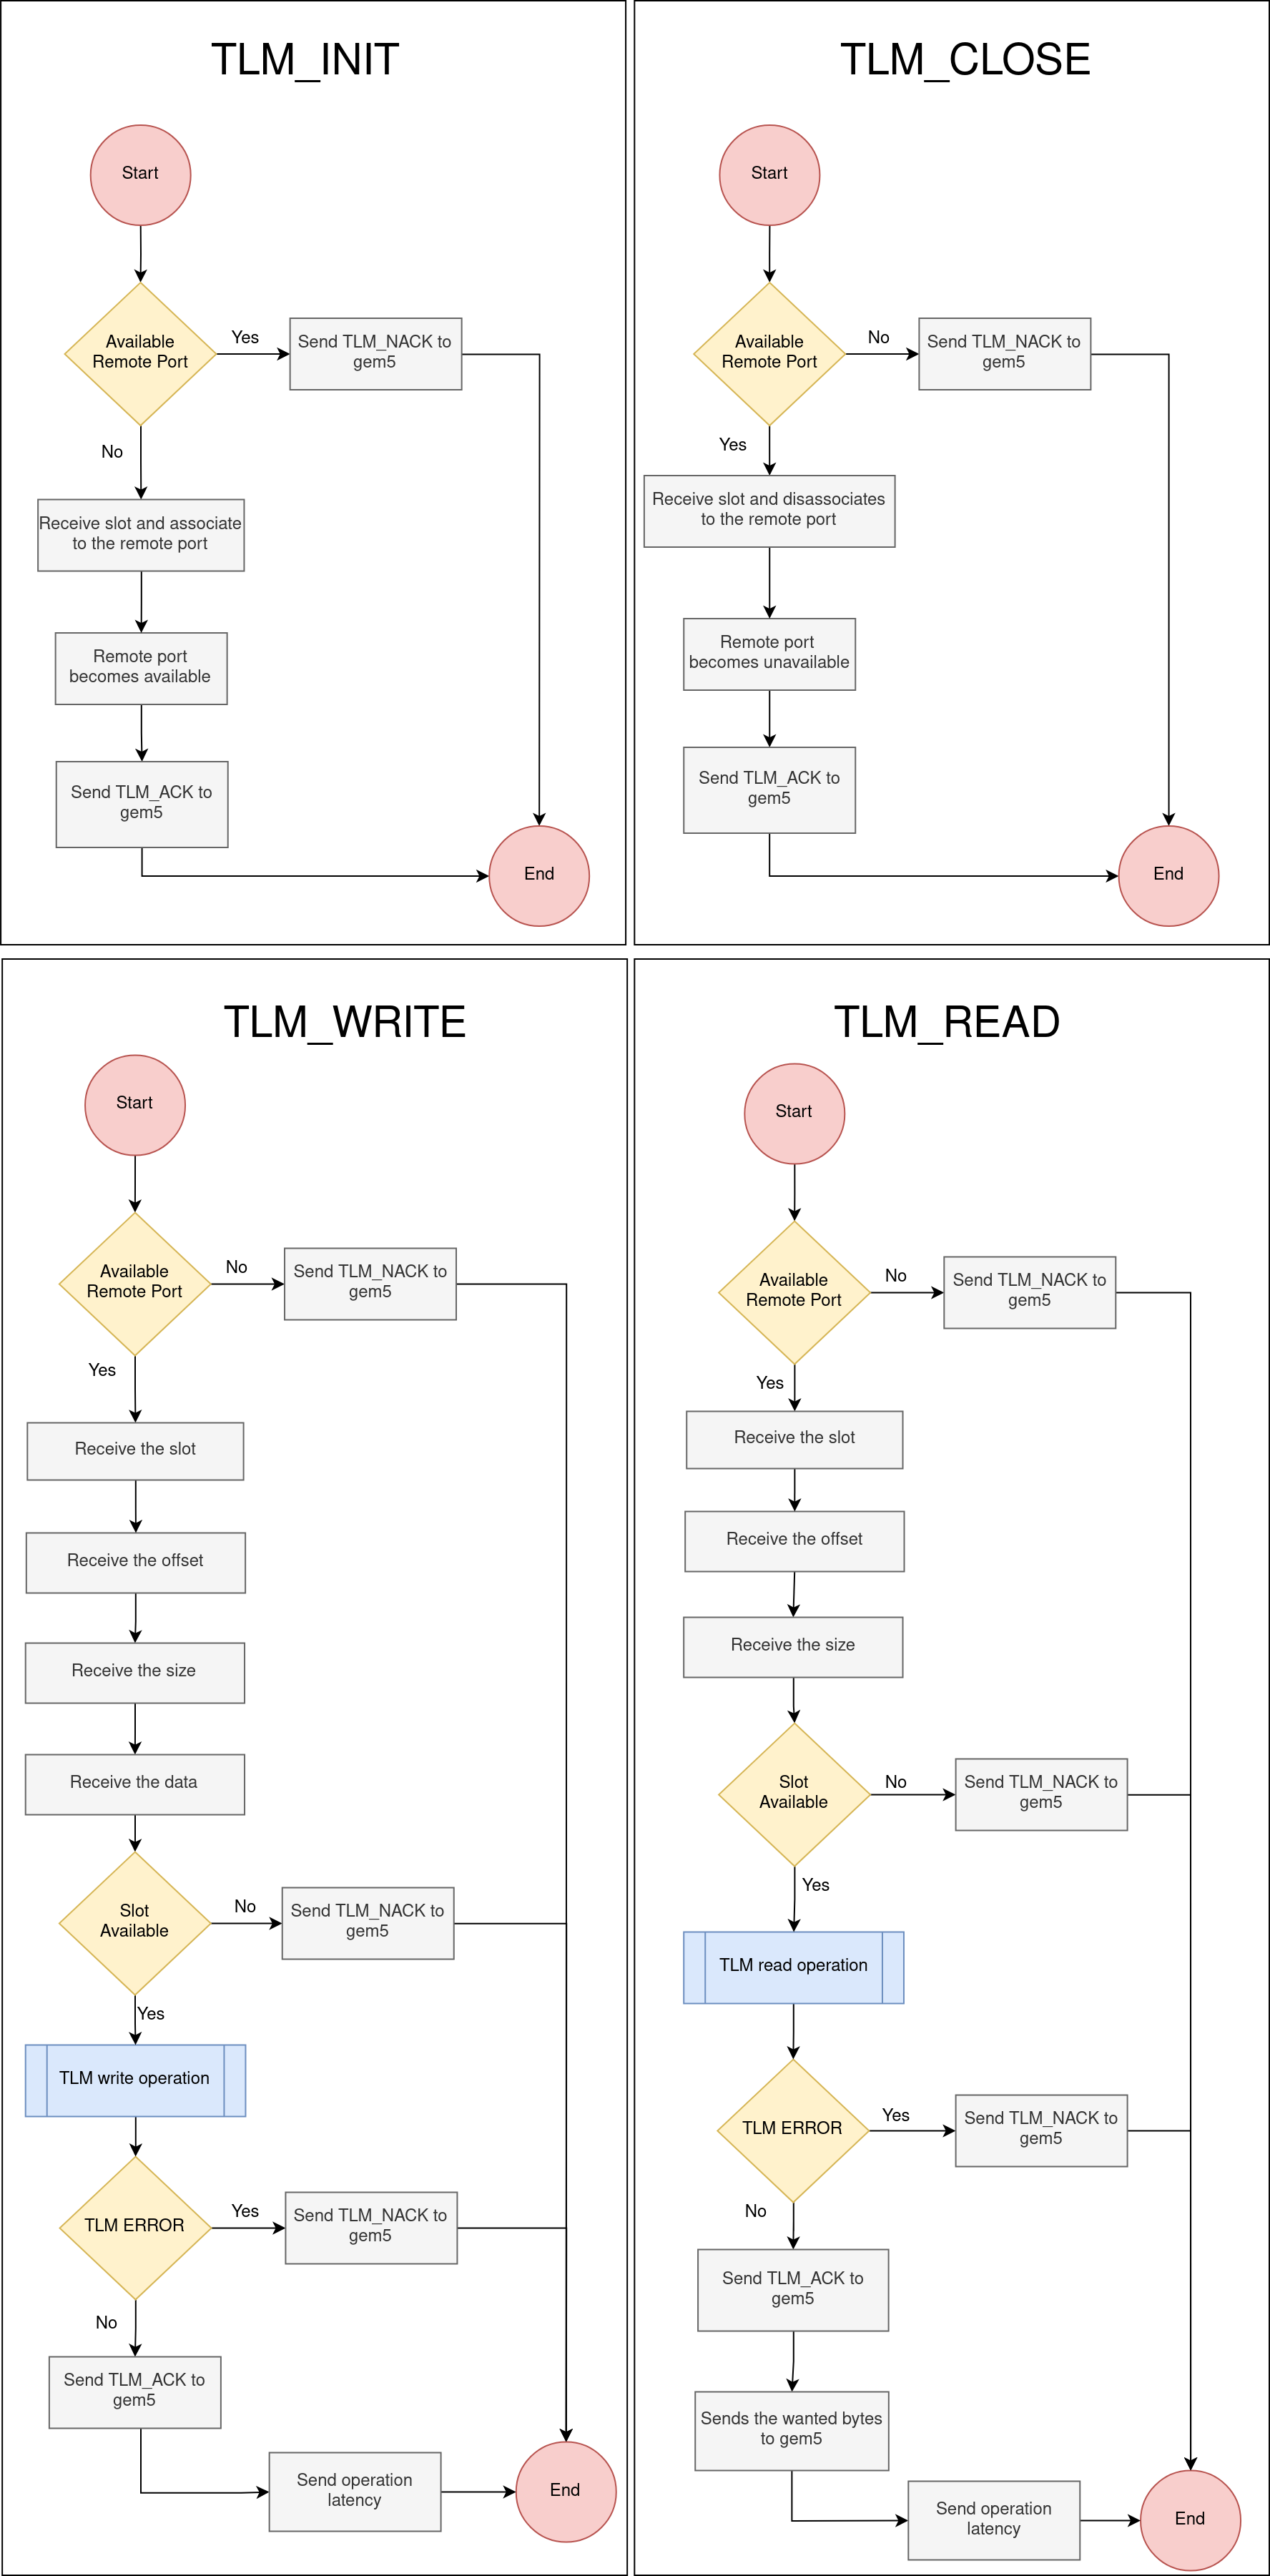
\includegraphics[width=0.7\linewidth]{Images/TLMWrapper_SystemC.png} 
 	\caption{TLM wrapper in SystemC}
	% \label{fig_TLM_Wrapper_Payload}
\end{figure}

In the end, the wrapper can be described as presented in the \autoref{fig_TLM_Wrapper_ClassDiagram}. \textit{TLM\_Socket} provides an abstraction 
for socket write and read processes. Both have a dependency relationship since the \textit{TLM\_Wrapper} depends on the 
\textit{TLM\_Socket} functions to be able to communicate. When a remote port is initialized, the socket identification number is returned, 
and it is stored in the \textit{data\_fd} variable. In this way, it is possible to associate the slot with the respective remote port, providing 
coherent communication. When closing the remote port, this variable is reset to its default value. 

\begin{figure}[!ht]
	\centering
 	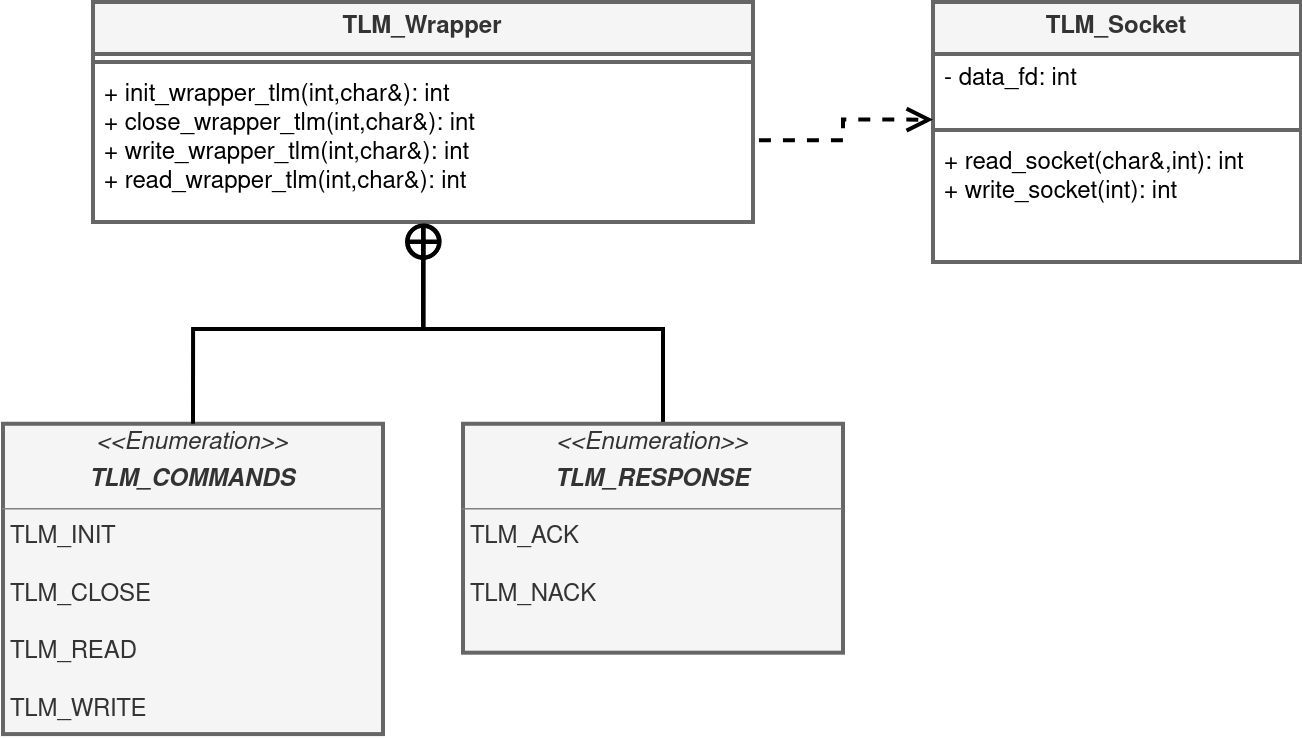
\includegraphics[width=0.7\linewidth]{Images/TLM_Wrapper_ClassDiagram.png} 
 	\caption{TLM wrapper class diagram}
	\label{fig_TLM_Wrapper_ClassDiagram}
\end{figure}

\subsection{SystemC Interface}

The peripheral development was carried out using the SystemC tool. It has the capability to simulate multiple and different hardware devices 
at the same time. In order to integrate this flexibility, the subsequent design was developed.

\begin{figure}[H]
	\centering
	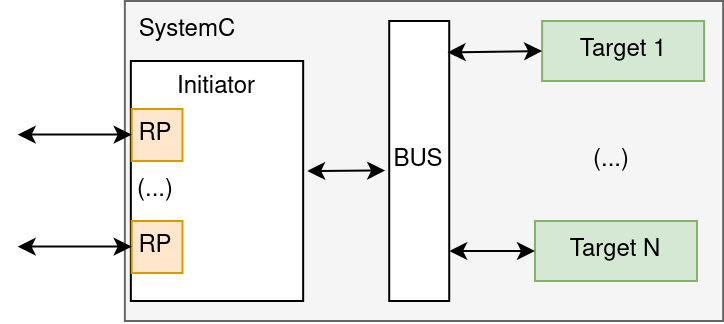
\includegraphics[width=0.6\textwidth]{Images/SystemCdesign.png}
	\caption{General SystemC design}
	\label{fig_SystemCdesign_geral}
\end{figure}


SystemC design is composed of three main components, which will communicate under the blocking transport method. 
The initiator, the bus, and the targets.
The first serves as the initial 
point of interaction for the tool since it handles incoming frames received through the remote port. The remote port operates independently 
of the initiator, enabling asynchronous reception and transmission of bytes through the receiver and transmit buffers, respectively.
Additionally, it also performs an interpretation of the received transaction and creates the \gls{tlm} transaction. It analyses various 
parameters such as the operation type, the desired target, and the memory region, among others, with the help of \textit{TLM\_wrapper}.

The bus is responsible for forwarding the \gls{tlm} transaction to the correct target. Each target has a unique ID, that is assigned 
at the beginning of the simulation. As previously mentioned, the preamble data and data were designed for a 32-bit architecture, however 
SystemC \gls{tlm} transactions are 64-bit width, leaving 32 bits unused. Before the transmission, the initiator uses these bytes to set the 
target ID, which will be utilized by the bus to identify the targets.

Lastly, the targets are the peripherals, which can be different from each other. These receive the 
\gls{tlm} commands and act accordingly. The next images demonstrate how peripherals respond to \textit{TLM\_READ} and \textit{TLM\_WRITE} operations. 

\begin{figure}[H]
	\centering
	\begin{subfigure}{\textwidth}
		\centering
		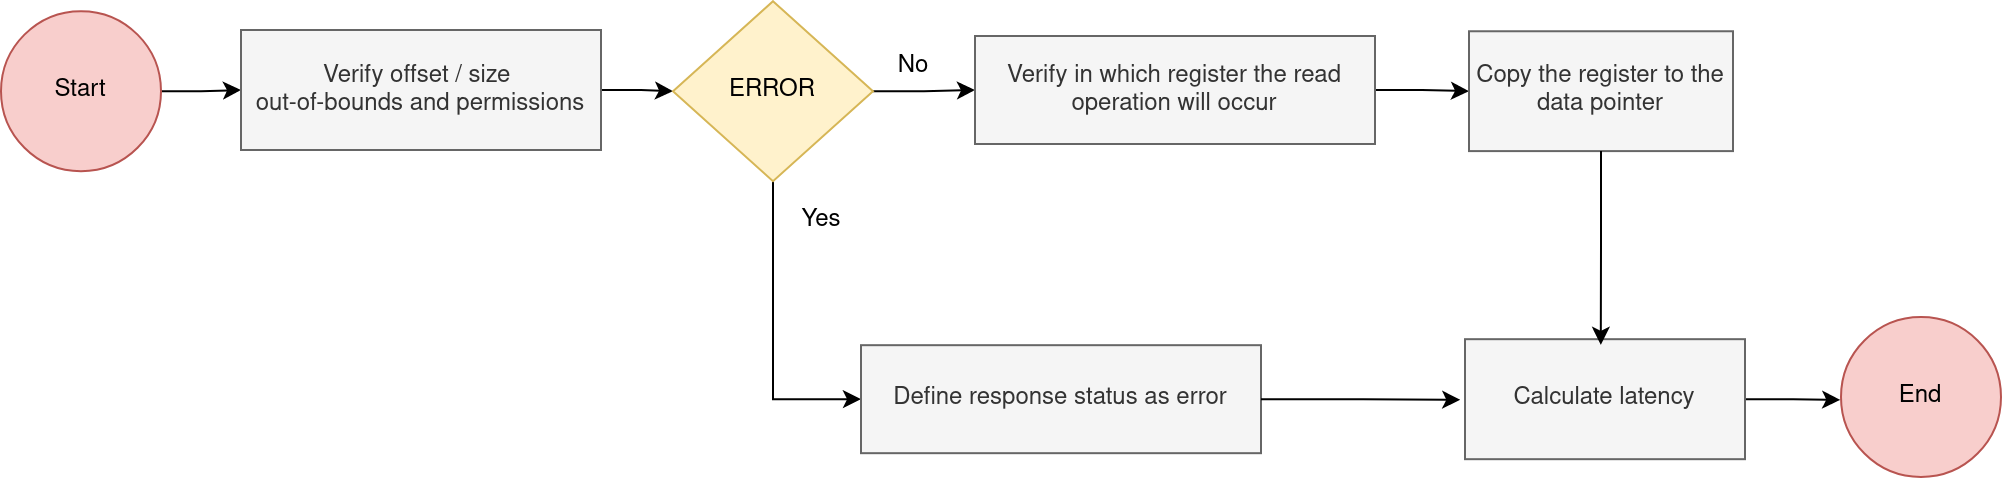
\includegraphics[width=0.9\textwidth]{Images/CoSimReadOperation.png}
 		\caption[1\textwidth]{Read command}
	\end{subfigure}
	\begin{subfigure}{\textwidth}
		\centering
		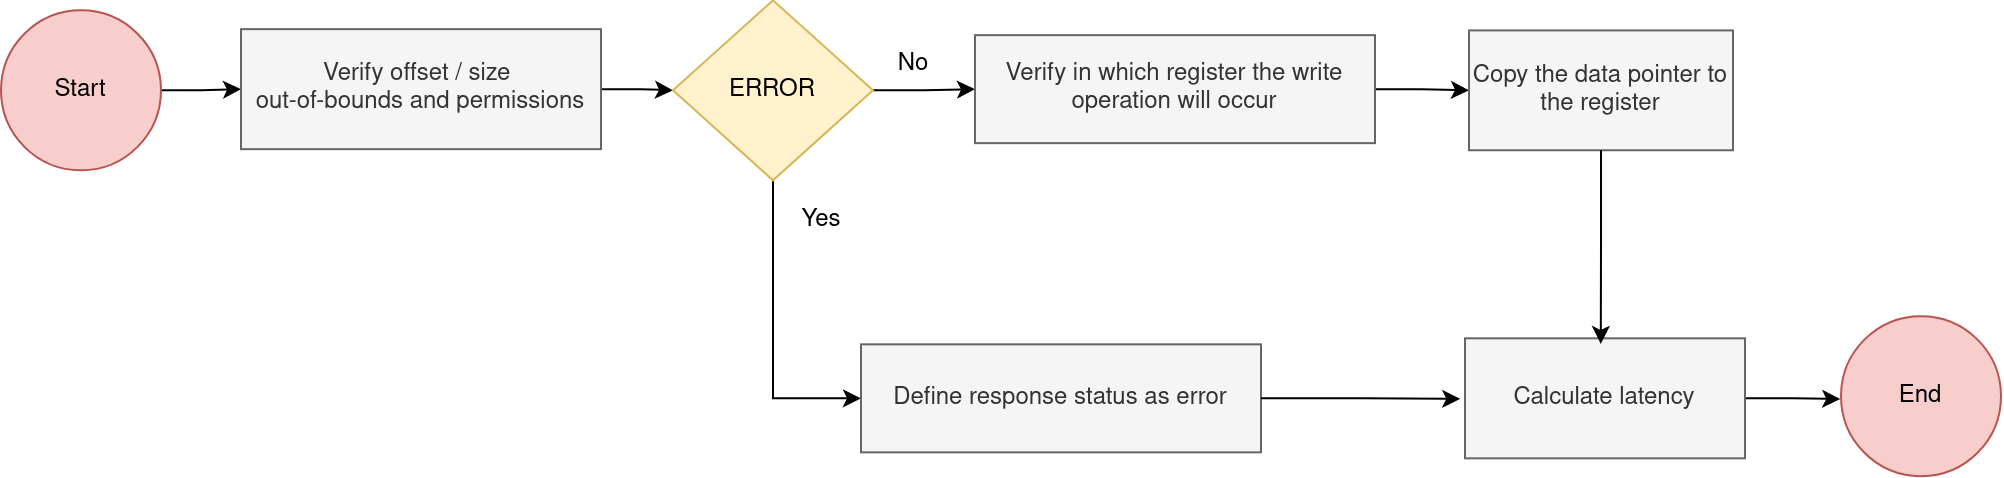
\includegraphics[width=0.9\textwidth]{Images/CoSimWriteOperation.png}
		\caption[1\textwidth]{Write command}
	\end{subfigure}
		
	\caption{Flowcharts of the available commands}
\end{figure}

The first step is to verify the offset/size out-of-bounds, and permissions in a way that the device's integrity is maintained. If no errors occurred 
in this process, the desired operation is done otherwise, an error response is created, reporting where the problem was. 
At the end of each operation, the correspondent latency is returned, which may vary regarding the desired work. The latency is used to inform the 
other simulator how long it should wait until a new operation can be done. An example concerning this can be seen in the above subsection.  

\subsection{Gem5 Interface}

Gem5 can integrate different boards with different characteristics. Nevertheless, the steps for integrating a device remain the same across 
all boards. 

The first step is the identification of available memory in the \gls{mcu}'s \gls{mmio}, and reserve the required memory for the device. 
Most microcontrollers have a lot of unused \gls{mmio} available, enabling the testing with new peripherals while retaining most of the 
original \gls{mcu}.

After planning this, Gem5 must recognize this hardware to enable communication with the other simulator. 
To achieve that, every peripheral should be defined and added to the list of off-chip devices in the 
board's configuration. In addition, it is also required to create a \gls{pte} for each device, which can be done by following the
code on \ref{templatePTE}. However, it's important to note that after this process, the devices are only recognized as part of the 
board, and their implementation still needs to be completed.

\hspace{1cm}

\begin{lstlisting}[style=customasm, caption={Template for a \gls{pte}}, label=templatePTE]
LDR   r1,= DEVICE_ADDR	 // Device address
LSR   r1, r1, #20        // Find which 1MB block it is in
LSL   r2, r1, #2         // Gives offset into the page tables
LSL   r1, r1, #20        // Put back in address format
LDR   r3, =L1_DEVICE     // Descriptor template
ORR   r1, r1, r3         // Combine address and template
STR   r1, [r0, r2]       // Store table entry
\end{lstlisting}


\begin{figure}[t!]
	\centering
	\begin{subfigure}{0.4\textwidth}
		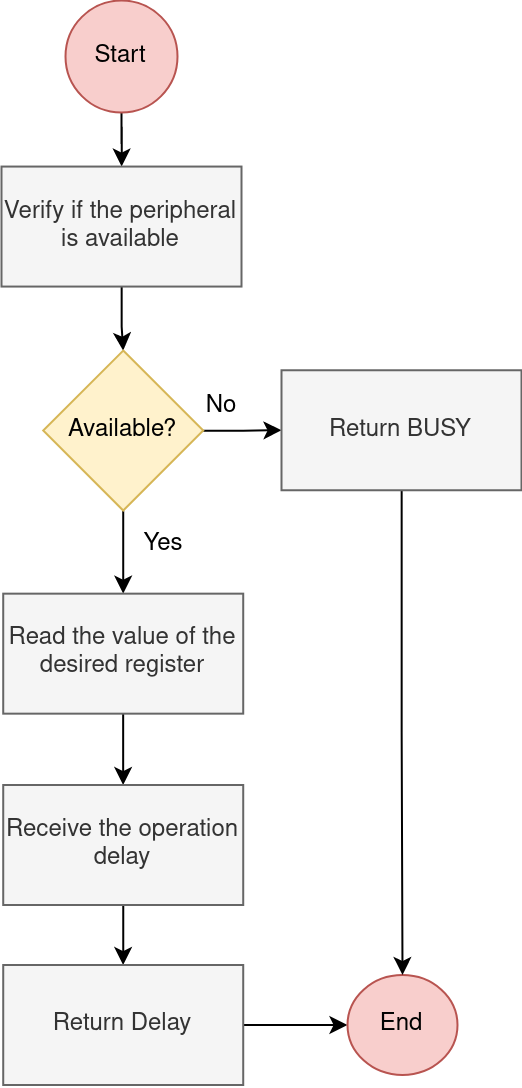
\includegraphics[width=0.7\textwidth]{Images/CrcReadFunction.png}
 		\caption[1\textwidth]{Device's read flowchart} 
	 	\label{fig_CrcReadFunction}
	\end{subfigure}
	\hspace{1cm}
	\begin{subfigure}{0.4\textwidth}
		\centering
		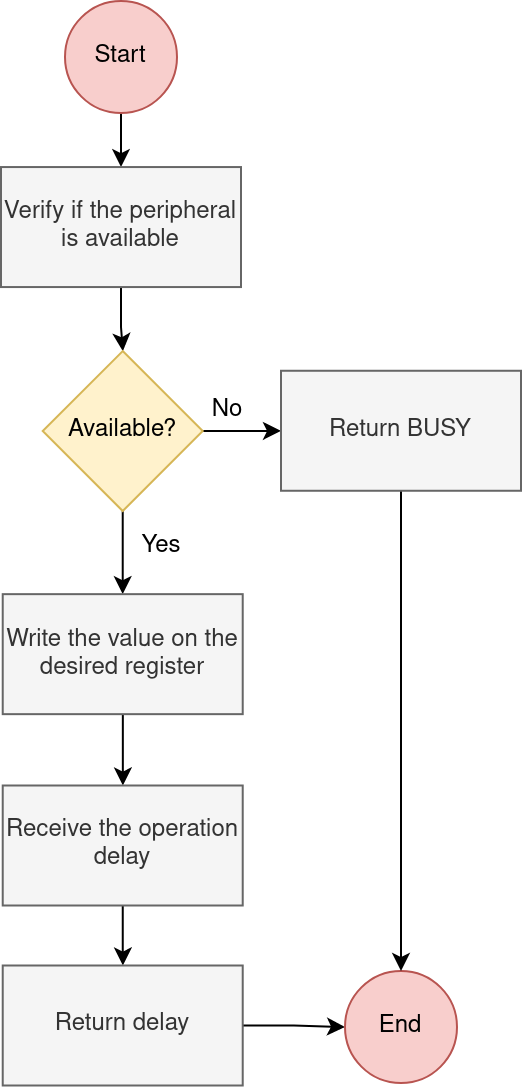
\includegraphics[width=0.7\textwidth]{Images/CrcWriteFunction.png}
		\caption[1\textwidth]{Device's write flowchart}
		\label{fig_CrcWriteFunction}
	\end{subfigure}
		
	\caption{Redefinition of \textit{BasicPioDevice} functions}
	\label{fig_Gem5ReadWrite}
\end{figure}
 
To implement a device in Gem5, a few aspects are mandatory. First of all, the peripheral interface, which describes the type, 
where the implementation is, and, optionally, some parameters to be customized. In this context, these can be
the port number, for the remote connection, or the action time delay. 
In second place, is the implementation itself. To accomplish this, the class \textit{BasicPioDevice} should be used. It is the base class 
which all devices sensitive to an address range inherit from. It abstracts all device's implementation, from the creation of the SimObject 
to memory access protocols. Still, it is required to define the read and write operations, as these change from device to device. 
The figures \ref{fig_CrcReadFunction} and \ref{fig_CrcWriteFunction} present a template for this implementation. Both start evaluating if
the peripheral is available or not. If it is negative, a busy notification is returned informing that it is not available at the 
moment. Otherwise, the respective operation is performed, returning the amount of time spent.

The last step is the connection to the remote port interface. The connection process is the following: Firstly, a socket must be created; 
After that, the simulator listens to the socket and waits until a connection is made; Finally, it verifies if the other interfaces are ready 
by initializing the co-simulation environment. If it receives a positive response, the simulation can proceed, else the simulation is aborted. 
Note that all this process is done before the actual benchmark starts. 

\section{CRC as a Case Study}

To stimulate the developed interface, the \gls{crc} peripheral was chosen as a case study.
This selection was based on its presence in several microcontroller families, such as STM32 \cite{referenceManualRM0385} or Xilinx Zynq \cite{xilinx2014zynq}.

The \gls{crc} was created in 1961 by William Wesley Peterson \cite{peterson1961cyclic}. As the name suggests, 
it utilizes systematic cyclic codes to encode messages by incorporating a fixed-length check value. In the end, his work
contributed significantly to simplifying and enhancing the detection of accidental errors/changes in communication 
networks. \gls{crc} uses a generator polynomial, which is known by the sender and receiver, and it is used to 
perform the calculation. There are different standards however, the most common ones are the CRC-8, CRC-12, CRC-16, 
CRC-32, and CRC-CCIT \cite{borrelli2001ieee}

Another application for the \gls{crc} is the storage integrity. Due to defective components or electromagnetic fields,
bits can change their value without notice. In the presented case study, this scenario will be explored, where 
the \gls{crc} peripheral is used to maintain a specific memory state and verify if there have been any changes. 
Furthermore, the board will not be only engaged in this operation, because in real-world scenarios, it has additional functionalities 
besides memory verification. Hence, as a proof-of-concept, parallel tasks will be included in the execution.

\subsection{Peripheral Development on SystemC}

The development of the \gls{crc} peripheral was done in SystemC, which took as a reference the STM32 microcontroller family's 
reference manual \cite{referenceManualRM0385}. As presented in the figure below, the \autoref{fig_SystemCdesign_geral} was redefined to 
the present case study. The initiator will only have one remote port associated since only one device will be simulated.

\begin{figure}[H]
	\centering
	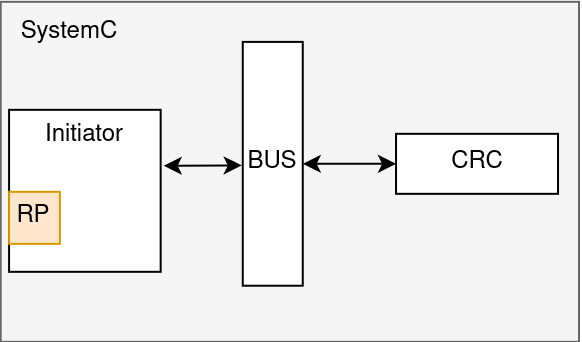
\includegraphics[width=0.5\textwidth]{Images/SystemCdesign_CRC.png}
	\caption{SystemC design with CRC}
	\label{fig_SystemCdesign_CRC}
\end{figure}

From the module datasheet, the peripheral is characterized by the following:  

\begin{itemize}
	\item CRC-32 (Ethernet) polynomial: 0x4C11DB7
	\item Programmable CRC initial value
	\item Single input/output 32-bit data register
	\item CRC computation done in 4 clock cycles 
	\item General-purpose 8-bit register (can be used for temporary storage)
	\item Reversibility option on I/O data
\end{itemize}

\begin{figure}[]
	\centering
 	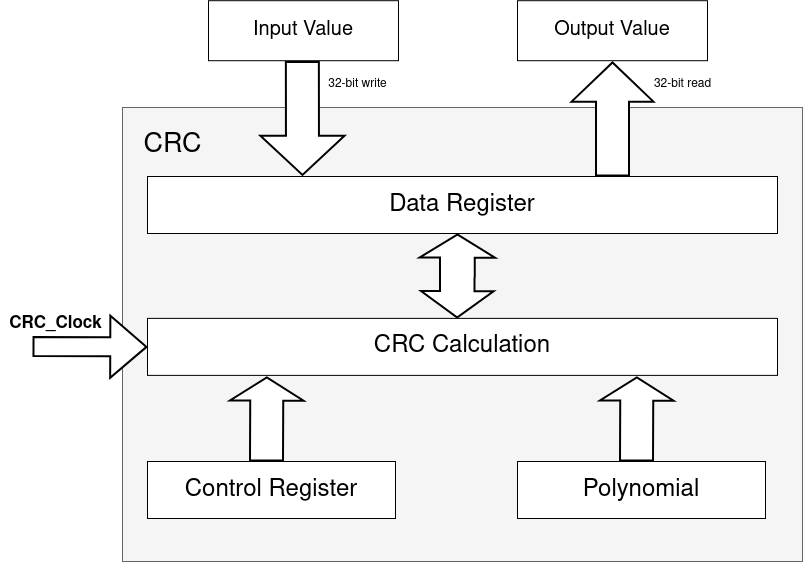
\includegraphics[width=0.65\linewidth]{Images/CrcBlockDiagram.png}
 	\caption{CRC block diagram}
	 \label{fig_CrcBlockDiagram}
\end{figure}


Regarding the \autoref{fig_CrcBlockDiagram}, the module working principle is as follows. First of all, the user needs to write the input value 
in the data register (CRC\_DR). After four \gls{crc} clock cycles, the correspondent \gls{crc} value is fully calculated, and its
value is stored in the CRC\_DR. In this case, the \gls{crc} frequency will be equal to the \gls{cpu}. The data width must be 32-bit, 
hence whether the user needs a \gls{crc} for five bytes, for example, two different computations will be needed. 

Moreover, the input and output data can be reversed, to manage the various endianness schemes. For the input data, the reverse operation 
is controlled by the REV\_IN[1:0] bits, and for the output data, the REV\_OUT bit is used. These, along with the reset bit, which is used to 
reset the \gls{crc}, are located in the control register (CRC\_CR). This bit must be set by software, and it is automatically cleared by
the hardware. An example of a reverse operation can be found on \autoref{tab:CRC_REV}.

\begin{table}[!htb]
    \caption{Reverse operation}
    \begin{minipage}{.5\linewidth}
      \centering
      \subcaption{Input}
		\resizebox{\textwidth}{!}{%
		\begin{tabular}{lllll}
		\cline{1-4}
		\multicolumn{1}{|l|}{\cellcolor[HTML]{C0C0C0}{\color[HTML]{000000} REV\_IN[1:0]}} & \multicolumn{1}{l|}{\cellcolor[HTML]{C0C0C0}{\color[HTML]{000000} Input}} & \multicolumn{1}{l|}{\cellcolor[HTML]{C0C0C0}{\color[HTML]{000000} Reverse Action}} & \multicolumn{1}{l|}{\cellcolor[HTML]{C0C0C0}{\color[HTML]{000000} Reverse Input}} &  \\ \cline{1-4}
		\multicolumn{1}{|l|}{0 0} & \multicolumn{1}{l|}{0x1A2B3C4D} & \multicolumn{1}{l|}{Not affected} & \multicolumn{1}{l|}{0x1A2B3C4D} &  \\ \cline{1-4}
		\multicolumn{1}{|l|}{0 1} & \multicolumn{1}{l|}{0x1A2B3C4D} & \multicolumn{1}{l|}{Bit-reversal done by byte} & \multicolumn{1}{l|}{0x58D43CB2} &  \\ \cline{1-4}
		\multicolumn{1}{|l|}{1 0} & \multicolumn{1}{l|}{0x1A2B3C4D} & \multicolumn{1}{l|}{Bit-reversal done by half-word} & \multicolumn{1}{l|}{0xD458B23C} &  \\ \cline{1-4}
		\multicolumn{1}{|l|}{1 1} & \multicolumn{1}{l|}{0x1A2B3C4D} & \multicolumn{1}{l|}{Bit-reversal done by word} & \multicolumn{1}{l|}{0xB23CD458} &  \\ \cline{1-4}
		&  &  &  & 
		\end{tabular}%
        }
        \label{tab:CRC_REV_IN}
    \end{minipage}%
    \begin{minipage}{.5\linewidth}
        \centering
        \subcaption{Output}
		\resizebox{\textwidth}{!}{%
		\begin{tabular}{lllll}
		\cline{1-4}
		\multicolumn{1}{|l|}{\cellcolor[HTML]{C0C0C0}{\color[HTML]{000000} REV\_OUT}} & \multicolumn{1}{l|}{\cellcolor[HTML]{C0C0C0}{\color[HTML]{000000} Output}} & \multicolumn{1}{l|}{\cellcolor[HTML]{C0C0C0}{\color[HTML]{000000} Reverse Action}} & \multicolumn{1}{l|}{\cellcolor[HTML]{C0C0C0}{\color[HTML]{000000} Reverse Output}} &  \\ \cline{1-4}
		\multicolumn{1}{|l|}{0} & \multicolumn{1}{l|}{0x11223344} & \multicolumn{1}{l|}{Not affected} & \multicolumn{1}{l|}{0x11223344} &  \\ \cline{1-4}
		\multicolumn{1}{|l|}{1} & \multicolumn{1}{l|}{0x11223344} & \multicolumn{1}{l|}{Bit-reversal done by word} & \multicolumn{1}{l|}{0x22CC4488} &  \\ \cline{1-4}
		 &  &  &  & 
		\end{tabular}%
        }   
        \label{tab:CRC_REV_OUT}
    \end{minipage}
	\label{tab:CRC_REV} 
\end{table}

By default, the polynomial coefficients are defined by 0x4C11DB7 nevertheless, it can be fully programmable through the CRC\_POL register.
It is important to mention that modifications in this register when a \gls{crc} computation is ongoing are not permitted, as it would 
compromise the output value. To complete the list of available registers, there are the CRC\_INIT and CRC\_IDR.  
These registers are used to initialize the \gls{crc} calculator during reset and to hold a temporary 8-bit value related to \gls{crc} 
calculation, respectively.

Finally, the write command must be redefined to adhere to the peripheral characteristics, as demonstrated in \autoref{fig_CRC_write}.
Since the read operation does not require a specific behavior depending on the desired registers, the aforementioned template does not demand any
action.   

\begin{figure}[ht!]
	\centering
 	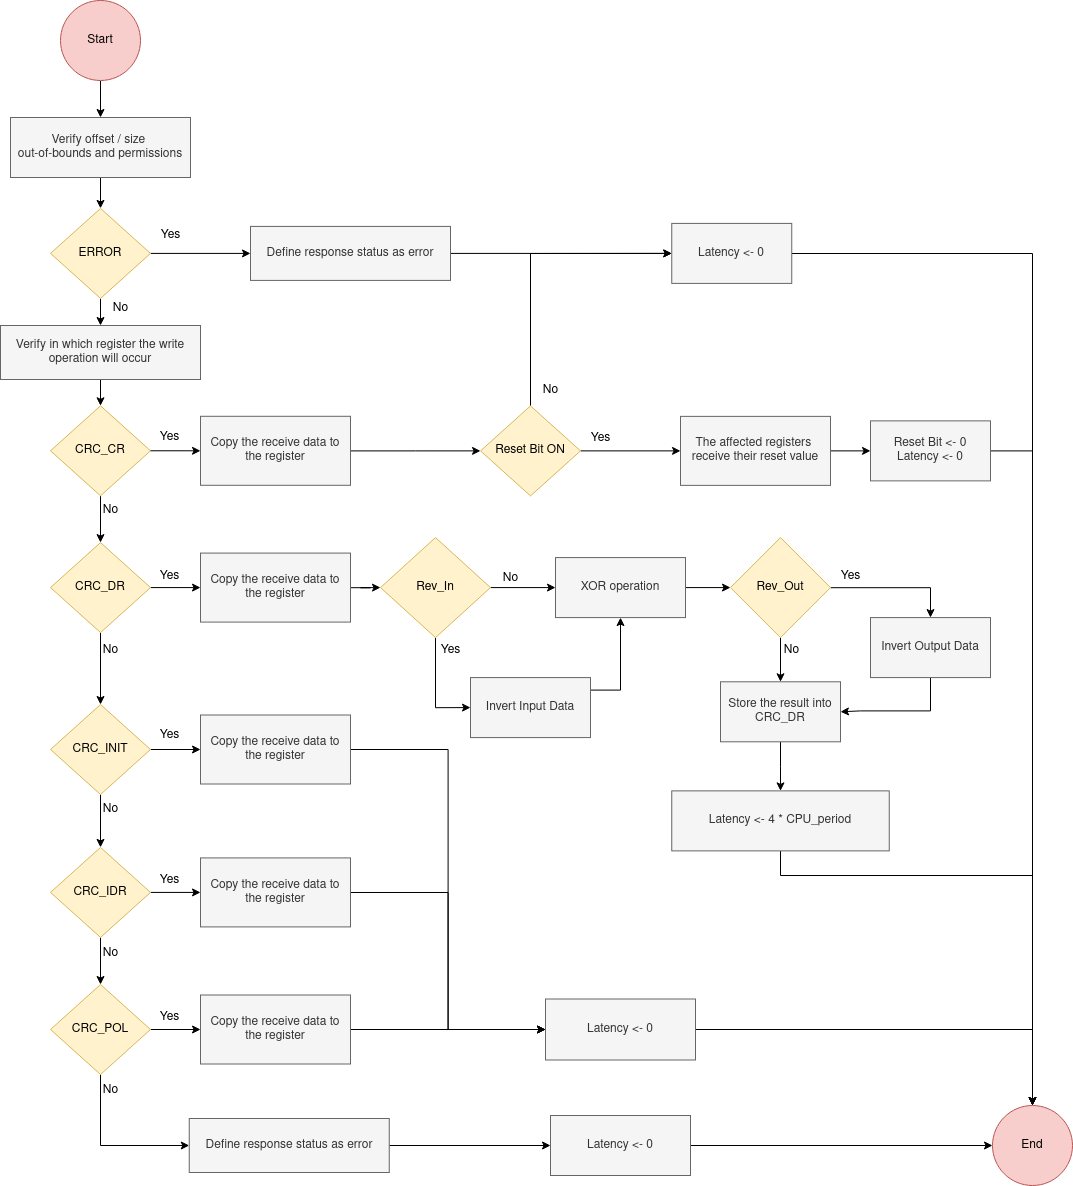
\includegraphics[width=0.7\linewidth]{Images/CRC_write.png}
 	\caption{CRC write operation}
	 \label{fig_CRC_write}
\end{figure}

\subsection{Peripheral Development on Gem5}

For the subsequent tests, the selected target platform was the VExpress\_gem5 board. It is based on the ARM Versatile Express RS1, which 
consists of a motherboard and two daughterboards. The system provides a range of both on-chip and off-chip devices.
On-chip devices include the Generic Interrupt Controller (GIC), an LCD controller, and system timers.
Off-chip devices contain the Keyboard and Mouse Interface (KMI), Real-Time Clock (RTC), and \gls{uart}. 
The platform's memory map is divided into the next sections.

\def\mydots{\xleaders\hbox to0.25em{\hfill.\hfill}\hfill}

\begin{outline}[enumerate]
	\1 Boot memory 						\mydots 	0x00000000 to 0x03FFFFFF
	\1 Reserved							\mydots 	0x04000000 to 0x0FFFFFFF
	\1 Off-chip peripherals				\mydots 	0x10000000 to 0x1FFFFFFF
		\2 Gem5-specific peripherals	\mydots 	0x10000000 to 0x13FFFFFF
			\3 Energy controller 		\mydots 	0x10000000 to 0x1000FFFF
			\3 Pseudo-ops				\mydots		0x10010000 to 0x1001FFFF
			\3 MHU						\mydots		0x10020000 to 0x1002FFFF
		\2 Reserved 					\mydots 	0x14000000 to 0x17FFFFFF
		\2 VRAM							\mydots		0x18000000 to 0x19FFFFFF
		\2 Reserved 					\mydots		0x1A000000 to 0x1BFFFFFF
		\2 Peripheral block 1			\mydots		0x1C000000 to 0x1FFFFFFF
	\1 On-chip  peripherals				\mydots 	0x20000000 to 0x3FFFFFFF
	\1 PCI memory 						\mydots 	0x40000000 to 0x7FFFFFFF
	\1 DRAM								\mydots 	0x80000000 to 0xFFFFFFFF
\end{outline}

The first aspect to take care of is the definition of the memory region. In accordance with the remaining devices, each peripheral should 
occupy 0xFFFF of memory space, unless it requires more space. In this case, another block of 0xFFFF should be used until its needs are fulfilled. 
Following the previously defined rule, for the understudy device memory will be reserved from 0x10030000 to 0x1003FFFF.

Then, the \gls{pte} entry must be created, with the \textit{DEVICE\_ADDR} parameter equal to the beginning of the device's memory, which 
is 0x10030000. The last part is the implementation of the write and read functions. Concerning the 
template present in the \autoref{fig_Gem5ReadWrite}, no modifications were needed to integrate this peripheral, therefore these were employed. 

\subsection{Application API}

At this point, the user on the application side can write and read directly from memory without any restriction. However, it can be
dangerous, in the way that the user can, by mistake, do an unpermitted operation. For example, write in reversed memory, causing a
segmentation fault. To avoid this, it was developed an \gls{api} for the application side. Similar to STM32 microcontrollers that 
utilize the HAL library, the \gls{crc} device will also have its own hardware abstraction layer. This layer is designed to speed up 
development and enhance code clarity.

\begin{figure}[H]
	\centering
 	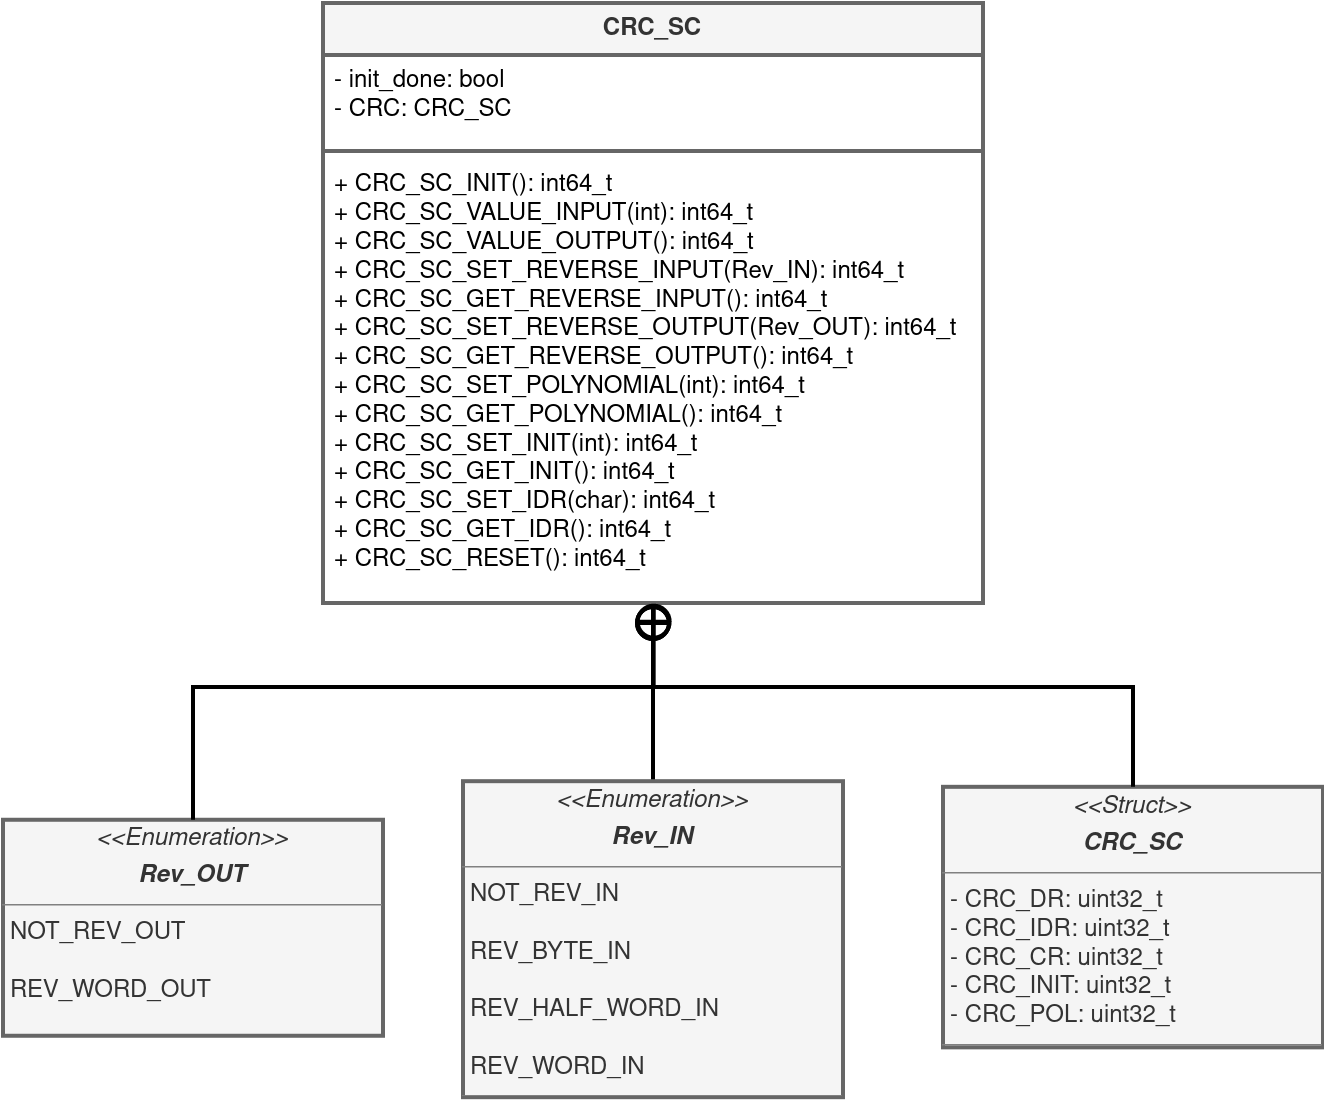
\includegraphics[width=0.7\linewidth]{Images/CRC_API_Class_Diagram.png} 
 	\caption{Class diagram for the CRC API}
	% \label{fig_TLM_Wrapper_Payload}
\end{figure}

Primarily, initializing the peripheral is a mandatory step. Without initialization, any attempt to execute an operation will 
result in an error, and no action will take place. To calculate the \gls{crc} value of a given number, the \textit{CRC\_SC\_VALUE\_INPUT} 
function must be called, with the corresponding number as a parameter. After that, the result can be obtained by calling the 
\textit{CRC\_SC\_VALUE\_OUTPUT} function. It is important to mention that the calculation takes four clock cycles, thus the function can 
either return the \gls{crc} result or an error, warning that the value is not calculated yet. All the remaining functions are used to
control the device.

\subsection{Peripheral Validation}

After development, the next step was to simulate and validate the peripheral. For this purpose, it was developed a validation test where
all features of the device will be tested. At the first moment, the device will be tested isolated, that is, without the remote port and Gem5 
interactions, as present in \autoref{fig_Validation_test_diagram}. After that, it will be tested in a co-simulation environment, as shown in the 
\autoref{fig_CoSimDesign_Validation}. 

\begin{figure}[H]
	\centering
 	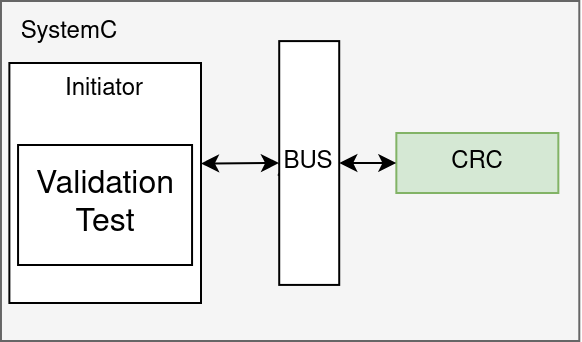
\includegraphics[width=0.5\linewidth]{Images/Validation_test_diagram.png} 
 	\caption{CRC peripheral validation}
	\label{fig_Validation_test_diagram}
\end{figure}

The designed validation test can be divided into three parts. In the first one, the reverse output will be tested. Then, the settings will 
change, and the calculation will use a reverse input and a different polynomial. To conclude, the reset function will be checked. 
By executing this benchmark, every functionality of the peripheral is checked. At the end of the simulation, the expected return values are 
0x22CC4488 for the first part and 0xC66CE444 for the second part. The final output will be the result of the reset operation. 

With this into account, the test was executed in the firstly mentioned condition, obtaining the results demonstrated in the figure below. As 
expected, the obtained results matched with the expected ones, concluding that the peripheral is working properly. 

\begin{figure}[H]
	\centering
 	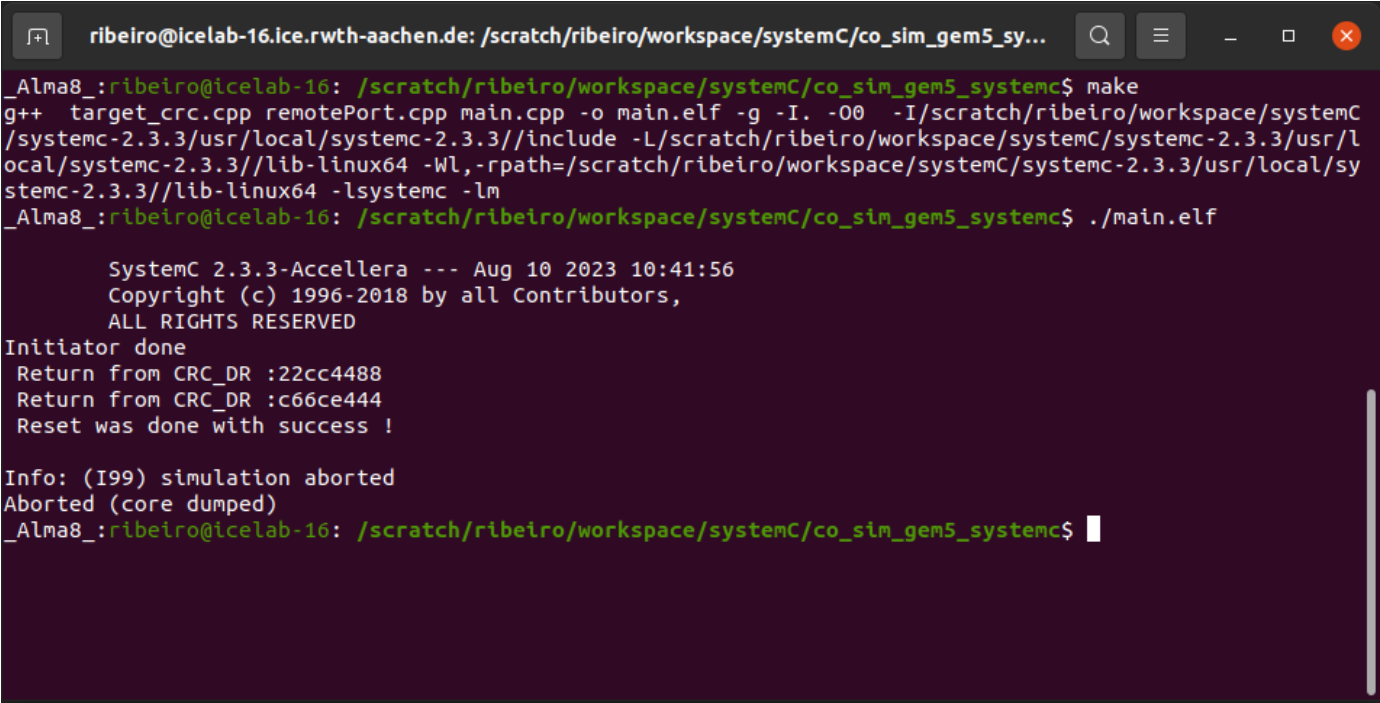
\includegraphics[width=0.9\linewidth]{Images/Validation_SystemC.png} 
 	\caption{CRC peripheral validation results}
\end{figure}

Moving to the co-simulation validation test, two cores will be employed in gem5's simulation for this purpose: one will be dedicated to the 
\gls{crc}, while the other will execute the bubble-sort benchmark. The simulation will be conducted in sequential mode since 
the main objective is not performance, but accuracy.

It will be used one \gls{crc} and the \gls{uart}, to communicate with the user by the terminal.
As referred, \gls{uart} is already implemented, hence it only requires its initialization and configuration. For the test, it will be used the 
\gls{uart}0, which is present in the memory map from 0x1C090000 to 0x1C09FFFF.
To connect to the \gls{uart}, the m5term can be utilized. It is
a dedicated program that allows the user to connect to the simulated console interface. When executing the simulation, this program does not
launch automatically, therefore it must be manually called, with \textit{./m5term <host> <port>}.

\begin{figure}[H]
	\centering
 	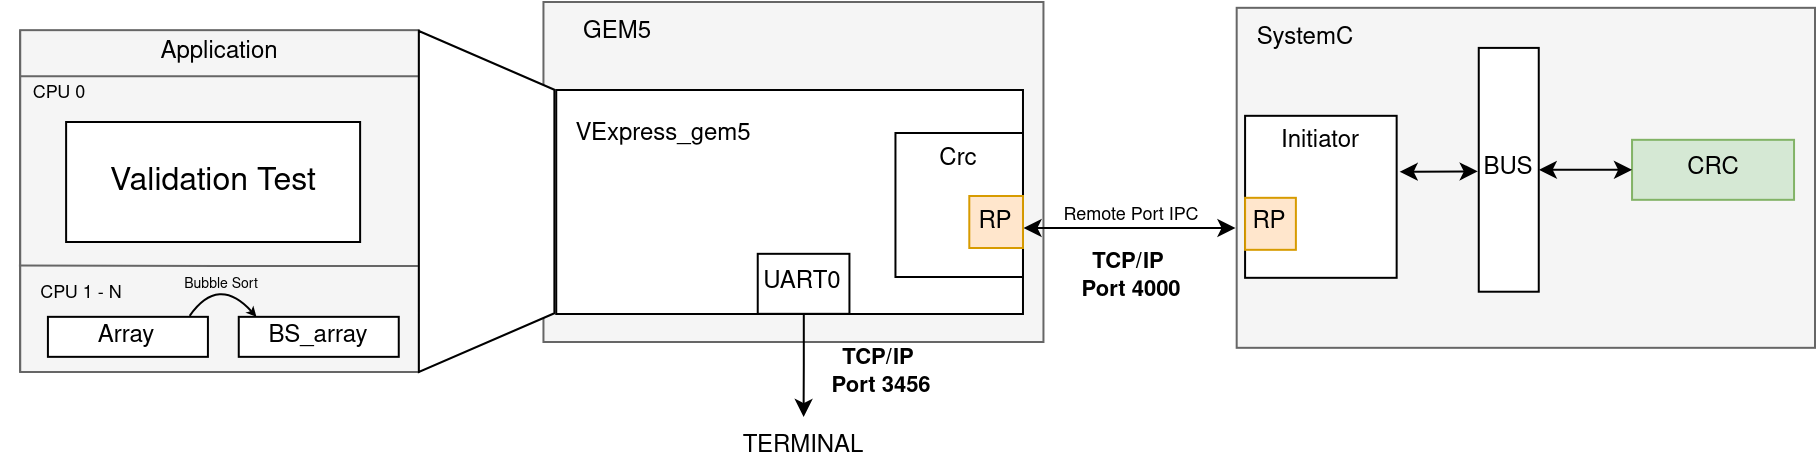
\includegraphics[width=1\linewidth]{Images/CoSimDesign_Validation.png} 
 	\caption{Validation co-simulation environment}
	\label{fig_CoSimDesign_Validation}
\end{figure}

The application will run the code present in \ref{validationCodeCRC}, which describes the previous validation test. 

\begin{lstlisting}[style=customC, caption={CRC validation code}, label=validationCodeCRC]
CRC_SC_INIT();

CRC_SC_SET_REVERSE_OUTPUT(REV_WORD_OUT);
CRC_SC_SET_IDR(0x4C);
CRC_SC_VALUE_INPUT(0x15e32ef3);       

do //Wait 4 tick
{
	CRC_value = CRC_SC_VALUE_OUTPUT();
} while (CRC_value == -EBUSY);

printf("Return from CRC_DR: %x \n", (uint32_t) CRC_value);

CRC_SC_SET_REVERSE_OUTPUT(NOT_REV_OUT);
CRC_SC_SET_REVERSE_INPUT(REV_HALF_WORD_IN);
CRC_SC_SET_POLYNOMIAL(0x12345678);
CRC_SC_VALUE_INPUT(0x1A2B3C4D);

do //Wait 4 tick
{
	CRC_value = CRC_SC_VALUE_OUTPUT();
} while (CRC_value == -EBUSY);

printf("Return from CRC_DR: %x \n", (uint32_t) CRC_value); 

CRC_SC_SET_INIT(0x4C11DB7);

if(CRC_SC_GET_IDR() == 0x4C)
	CRC_SC_RESET();

if(CRC_SC_VALUE_OUTPUT() == CRC_SC_GET_POLYNOMIAL())
	printf("Reset was done with success! \n");
else
	printf("Failure in Reset \n");

break;
\end{lstlisting}

After executing the validation benchmark, the real results were the ones present in the \autoref{fig_Validation_Results}. It is possible to 
conclude that the peripheral passed the validation since every expected output matches the real ones. 

\begin{figure}[H]
	\centering
 	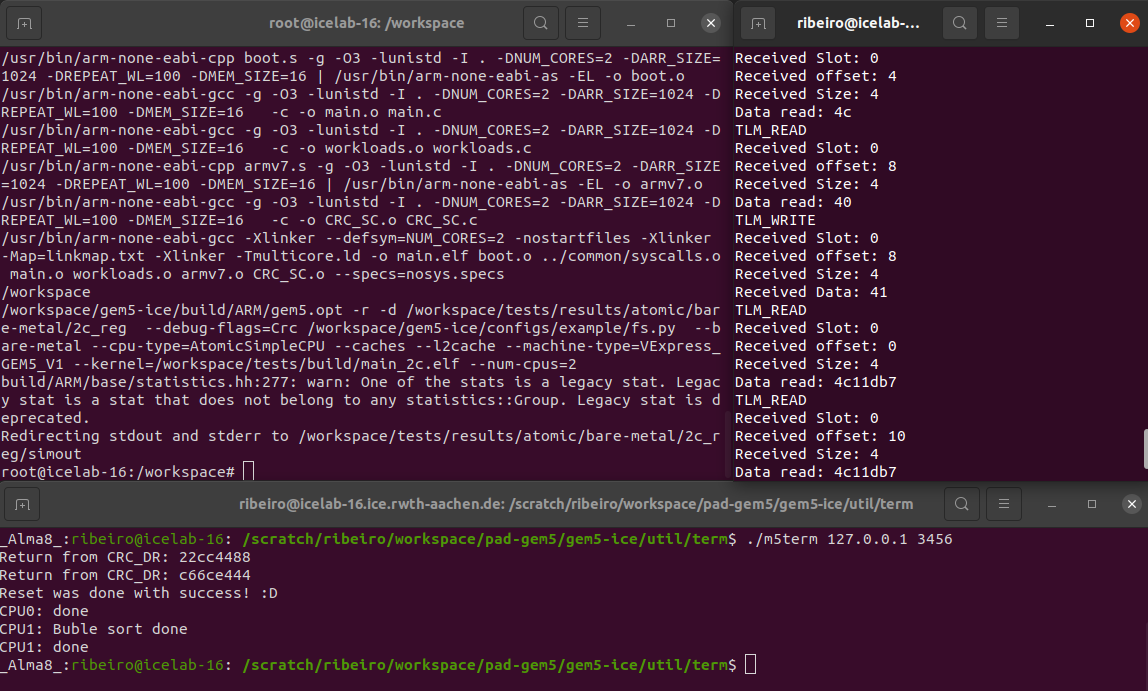
\includegraphics[width=0.8\linewidth]{Images/Validation_Results.png} 
 	\caption{Co-simulation environment validation results}
	\label{fig_Validation_Results}
\end{figure}


\subsection{Memory Integrity}

With the \gls{crc}'s validation, it is possible to simulate the scenario described at the beginning of this section. 
Similar to the validation test, 
from the application point of view, the system will execute 2 distinct jobs. \gls{cpu}0 will be responsible for 
performing the memory integrity checks, while the remaining ones will execute a bubble sort algorithm, as presented in 
the \autoref{fig_CoSimDesign}.

\begin{figure}[H]
	\centering
 	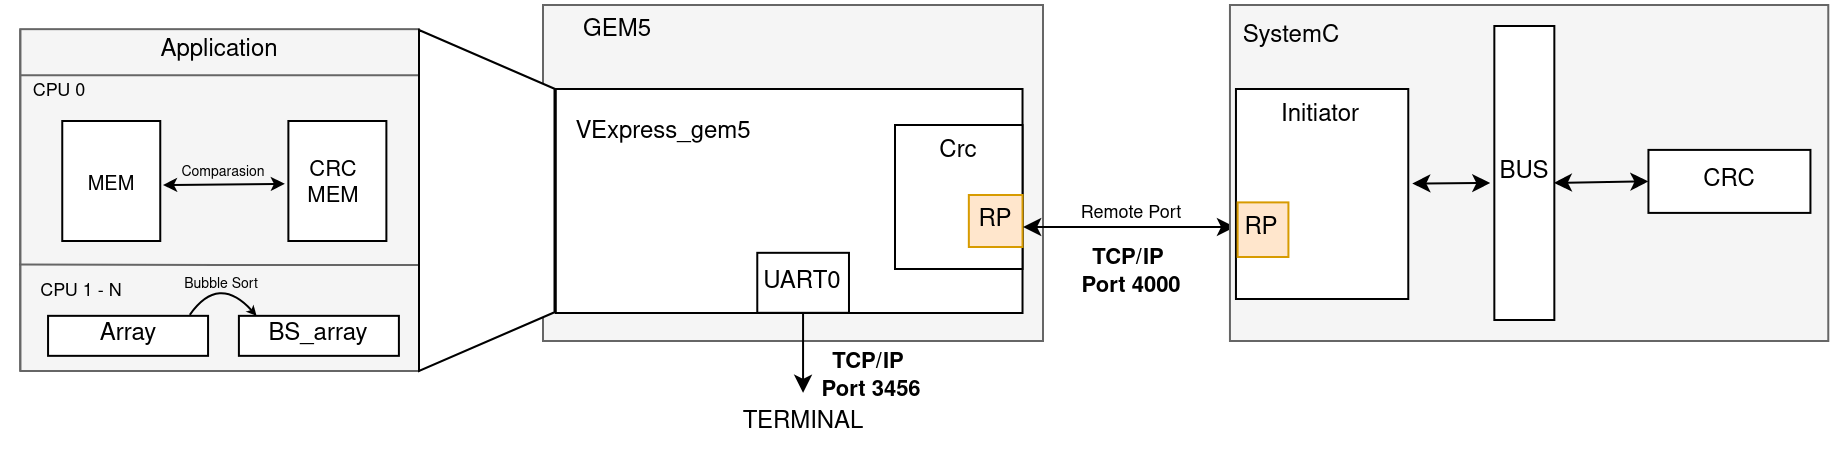
\includegraphics[width=1\linewidth]{Images/CoSimDesign.png}
 	\caption{Case study co-simulation environment}
	 \label{fig_CoSimDesign}
\end{figure}

When the benchmark starts, there is the creation of the intended \glspl{cpu}. Each one has an ID, that allows one to identify
themselves. To conduct the memory integrity test, \gls{cpu}0 will start initializing the \gls{crc} and the memory that will 
be utilized to compare. Afterward, periodically, it will perform a memory comparison, having two possible outcomes. Or everything
is all right, and the operation is a success. Or there is a flaw and the simulation ends immediately. A detailed view can be 
observed in \ref{fig_MemoryIntegrity_CPU0SequenceDiagram}. 

\begin{figure}[H]
	\centering
 	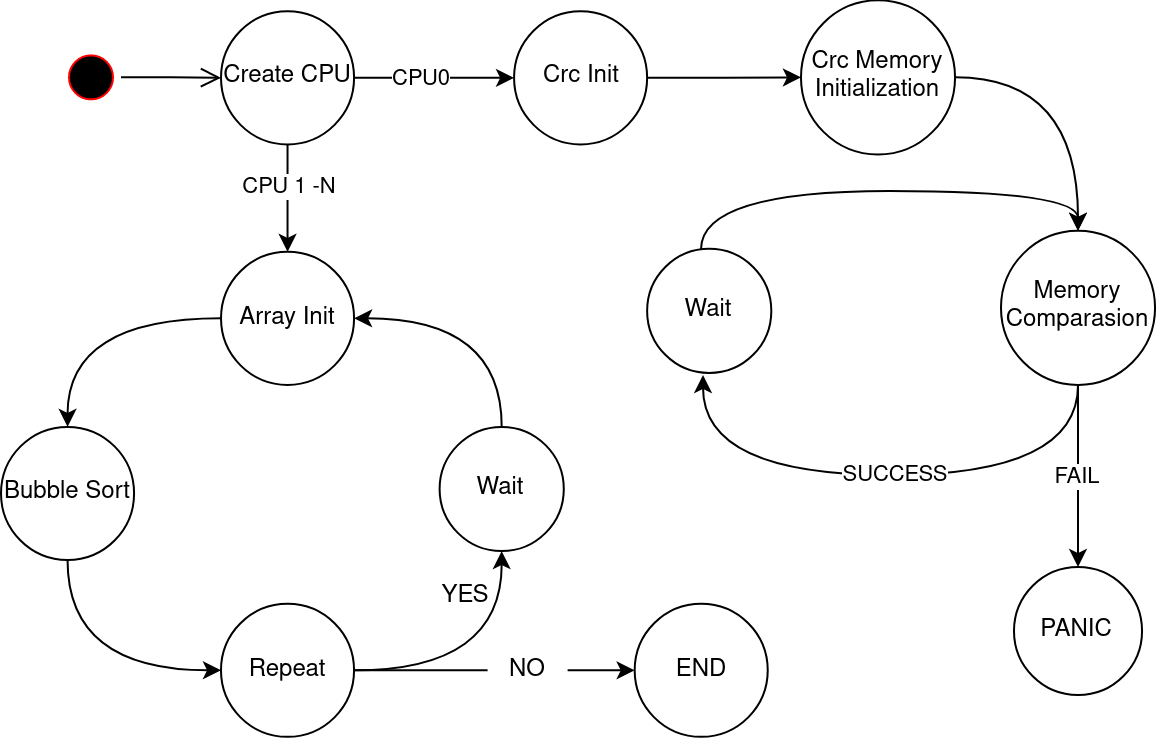
\includegraphics[width=0.7\linewidth]{Images/MemoryIntegrity_StateDiagram.png}
 	\caption{State machine diagram for the memory integrity test}
	\label{fig_MemoryIntegrity_StateDiagram}
\end{figure}

The bubble-sort test run in the remaining instaciated cores. Detail information about this benchmark can be found on \autoref{cap:BM}.
If its workload is concluded successfully and still there are memory verifications to carry out, the simulation continues since 
the primary objective is not to evaluate the bubble-sort algorithm. 


\begin{figure}[H]
	\centering
 	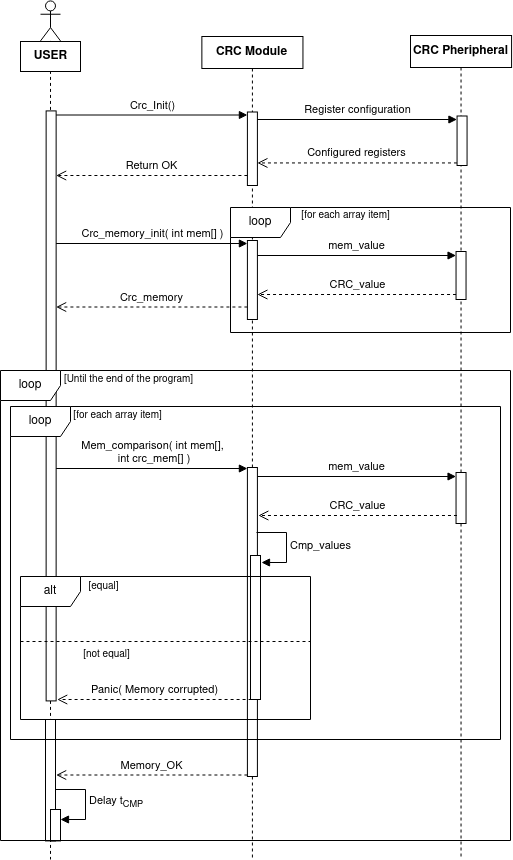
\includegraphics[width=0.7\linewidth]{Images/MemoryIntegrity_CPU0SequenceDiagram.png}
 	\caption{Sequence diagram diagram for the memory comparison}
	\label{fig_MemoryIntegrity_CPU0SequenceDiagram}
\end{figure}

\textbf{Success Modeling}
\newline

In the first memory integrity test, the perfect scenario will be simulated, in other words, the memory will operate without any failures, 
ensuring a well-functioning system. As represented in the \autoref{fig_MemoryIntegrity_StateDiagram}, there will be an interval between both 
tasks, and this can be different from each other (\ref{fig_AppTimeDiagram}). 

\begin{figure}[H]
	\centering
 	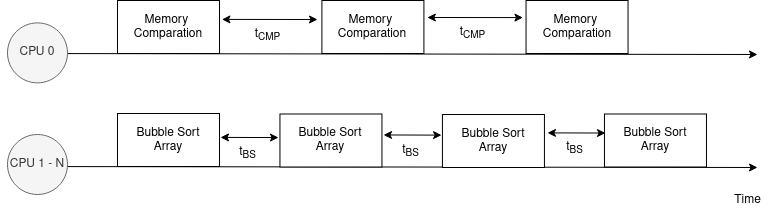
\includegraphics[width=0.8\linewidth]{Images/AppTimeDiagram.png}
 	\caption{Application execution timely diagram}
	 \label{fig_AppTimeDiagram}
\end{figure}


To perform this benchmark, the following parameters were defined. After completing the bubble-sort workload, the system executes a final 
memory check to ensure that no problems occurred between the last one, allowing the simulation to conclude safely. The simulation results are 
available in the subsequent images. As expected, the system executed normally the benchmark without any problems. Both \glspl{cpu} conclude the 
designated tasks and the last memory comparison gives positive feedback. 

\hspace{1.5cm}

\begin{multicols}{2}
	
	\begin{itemize}
		\item Repeat = 100
		\item $t_{CMP}$ = 100 ms
		\item $t_{BS}$ = 10 us
		\item Number of simulated cores = 2
		\item Memory size = 16
	\end{itemize}

	\columnbreak

	\begin{itemize}
		\item Simulation mode = sequential
		\item Reverse input \gls{crc} = REV\_HALF\_WORD\_IN
		\item Reverse output \gls{crc} = REV\_WORD\_OUT
		\item Polynomial = 0x04C11DB7
	\end{itemize}

\end{multicols}


\begin{figure}[H]
	\centering
 	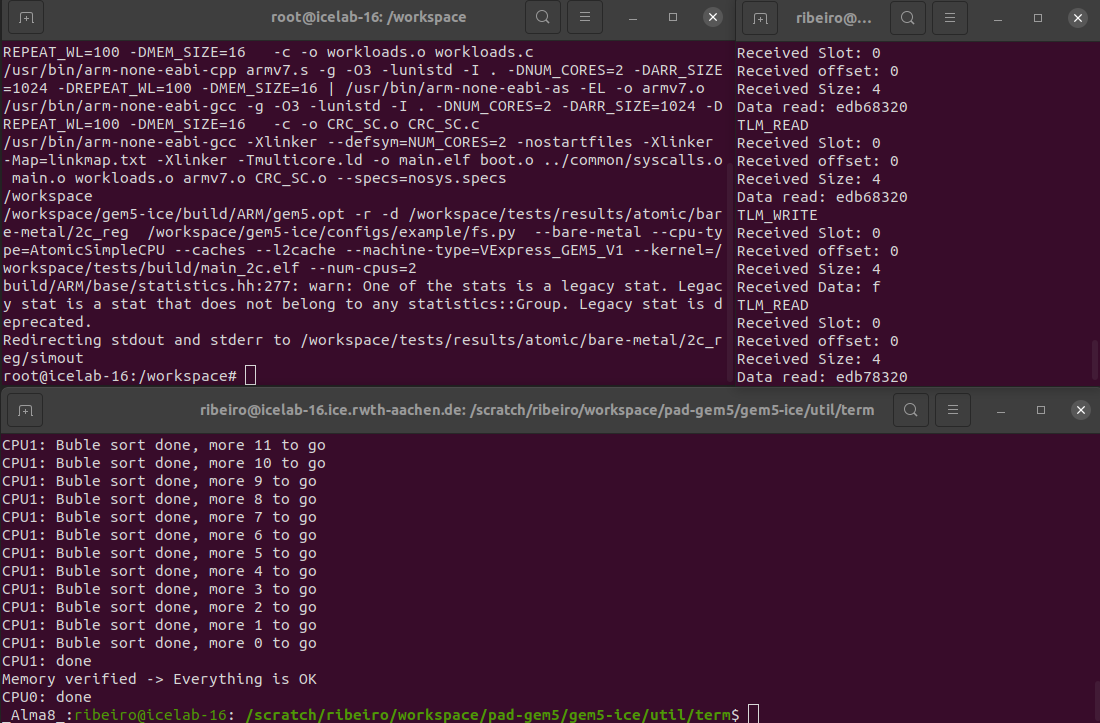
\includegraphics[width=0.8\linewidth]{Images/Success_MemoryIntegrity.png} 
 	\caption{Success memory integrity test}
	%\label{fig_Validation_Results}
\end{figure}


\textbf{Fault Modeling}
\newline

In opposition to the first, this test will simulate a corrupted memory scenario, as shown in the \autoref{fig_AppTimeDiagramFailure}. 
In order to achieve that, a failure will be injected into the memory with the \gls{gdb} tool. \gls{gdb} is a debugger 
that is supported by Gem5 and SystemC. It offers a variety of features but, for this purpose, the \textit{set var} command will be utilized. 
This command allows a value modification of a variable in real-time thus, in this way, the failure can be simulated.

\begin{figure}[H]
	\centering
 	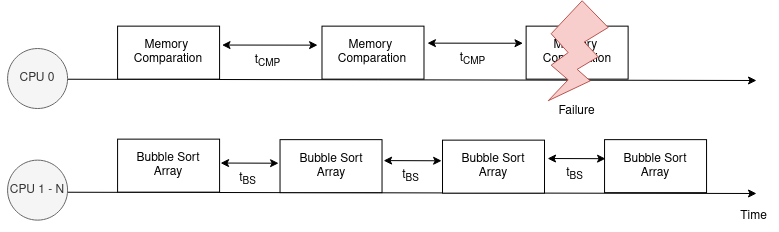
\includegraphics[width=0.8\linewidth]{Images/AppTimeDiagramFailure.png}
 	\caption{Application execution timely diagram with a failure}
	 \label{fig_AppTimeDiagramFailure}
\end{figure}


The test will be done under the same conditions as the previous one nevertheless, in this case, for comprehensive debugging capabilities, 
the debug version of the gem5 binary will be employed. In the end, the workload is expected to finish with an error from Gem5, and it can occur 
in two different moments. Either when the \gls{cpu}1-N are still running, or when these already completed their tasks. Both cases  
will be tested, and in either case, the program should terminate promptly. The \autoref{fig_Failure_MemoryIntegrity} demonstrates the obtained 
results, and it can be concluded that the system behaves in accordance with expectations.

\begin{figure}[!b]

	\centering
	\begin{subfigure}{\textwidth}
		\centering
		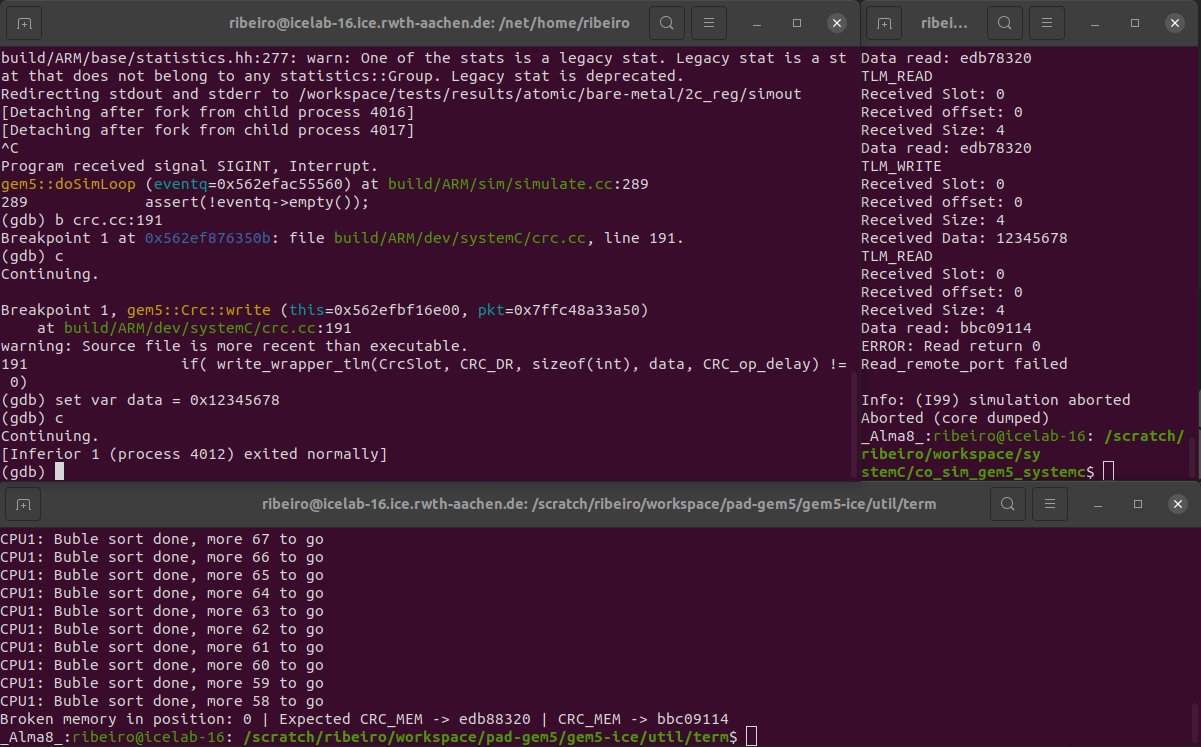
\includegraphics[width=0.8\textwidth]{Images/Failure_MemoryIntegrity1.png}
		\caption{Case 1}
	\end{subfigure}
\end{figure}
\begin{figure}[ht] \ContinuedFloat
	\begin{subfigure}{\textwidth}
		\centering
		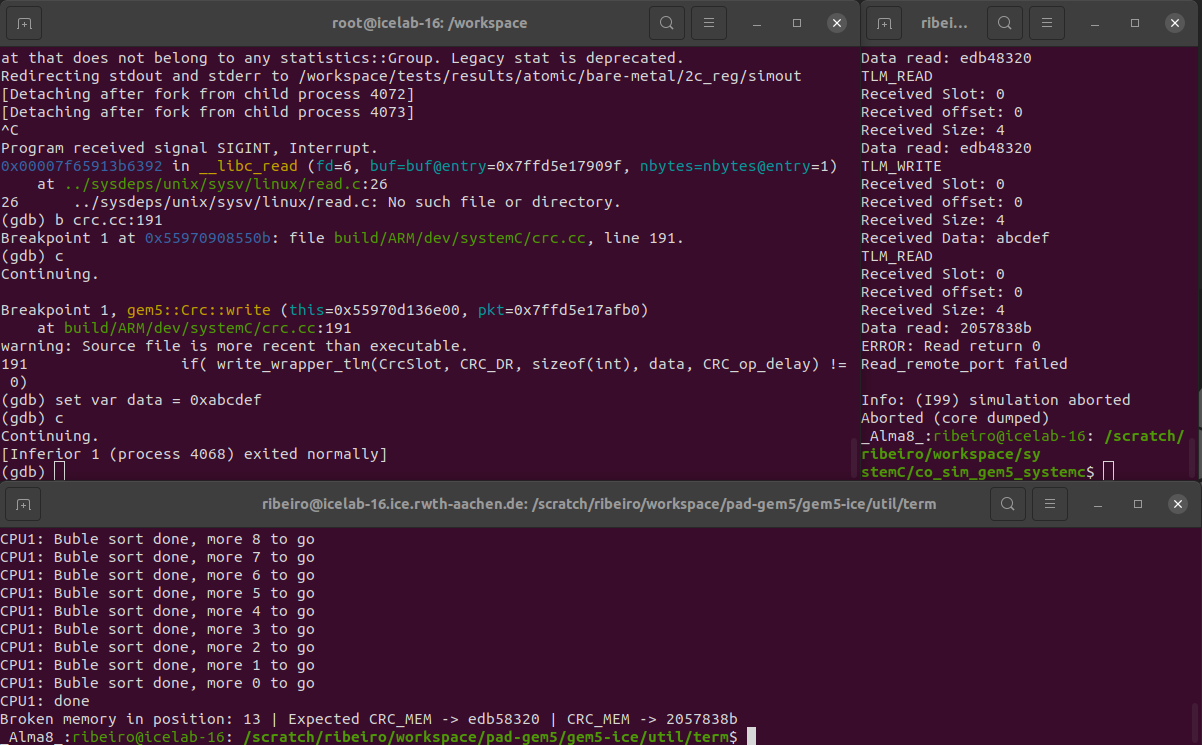
\includegraphics[width=0.8\textwidth]{Images/Failure_MemoryIntegrity2.png}
		\caption{Case 2}
	\end{subfigure}

	\caption{Failure memory integrity test}
	\label{fig_Failure_MemoryIntegrity}
\end{figure}


\section{Dynamic Quantum Integration}

Up to this point in the co-simulation, accuracy has been the primary concern. With this criteria, performance is sacrificed, giving a higher
host time. In the co-simulation itself, the use of par-gem5 would not provide greater benefits, as communication between the tools 
is the most time-consuming aspect. On the other hand, the remaining workload would take advantage of the parallel mode, as verified in the 
previous chapter (\ref{subsec::finalAlgorithm}). 

To assess the advantages of par-gem5 and the dynamic quantum during co-simulation, a series of tests were conducted with various configurations. 
Compared to the prior ones, the differences will be resumed to the simulation modes, with the addition of static and dynamic parallel modes, 
and the number of simulated cores, which will range from 2, 4, 8, 16, 32, to 64 cores. Further, the same setup of the previous section was used  
to perform this new set of tests (\autoref{fig_CoSimDesign}). The next figures exhibit the results obtained. 


\begin{figure}[]
	\centering
	\begin{subfigure}{\textwidth}
		\centering
		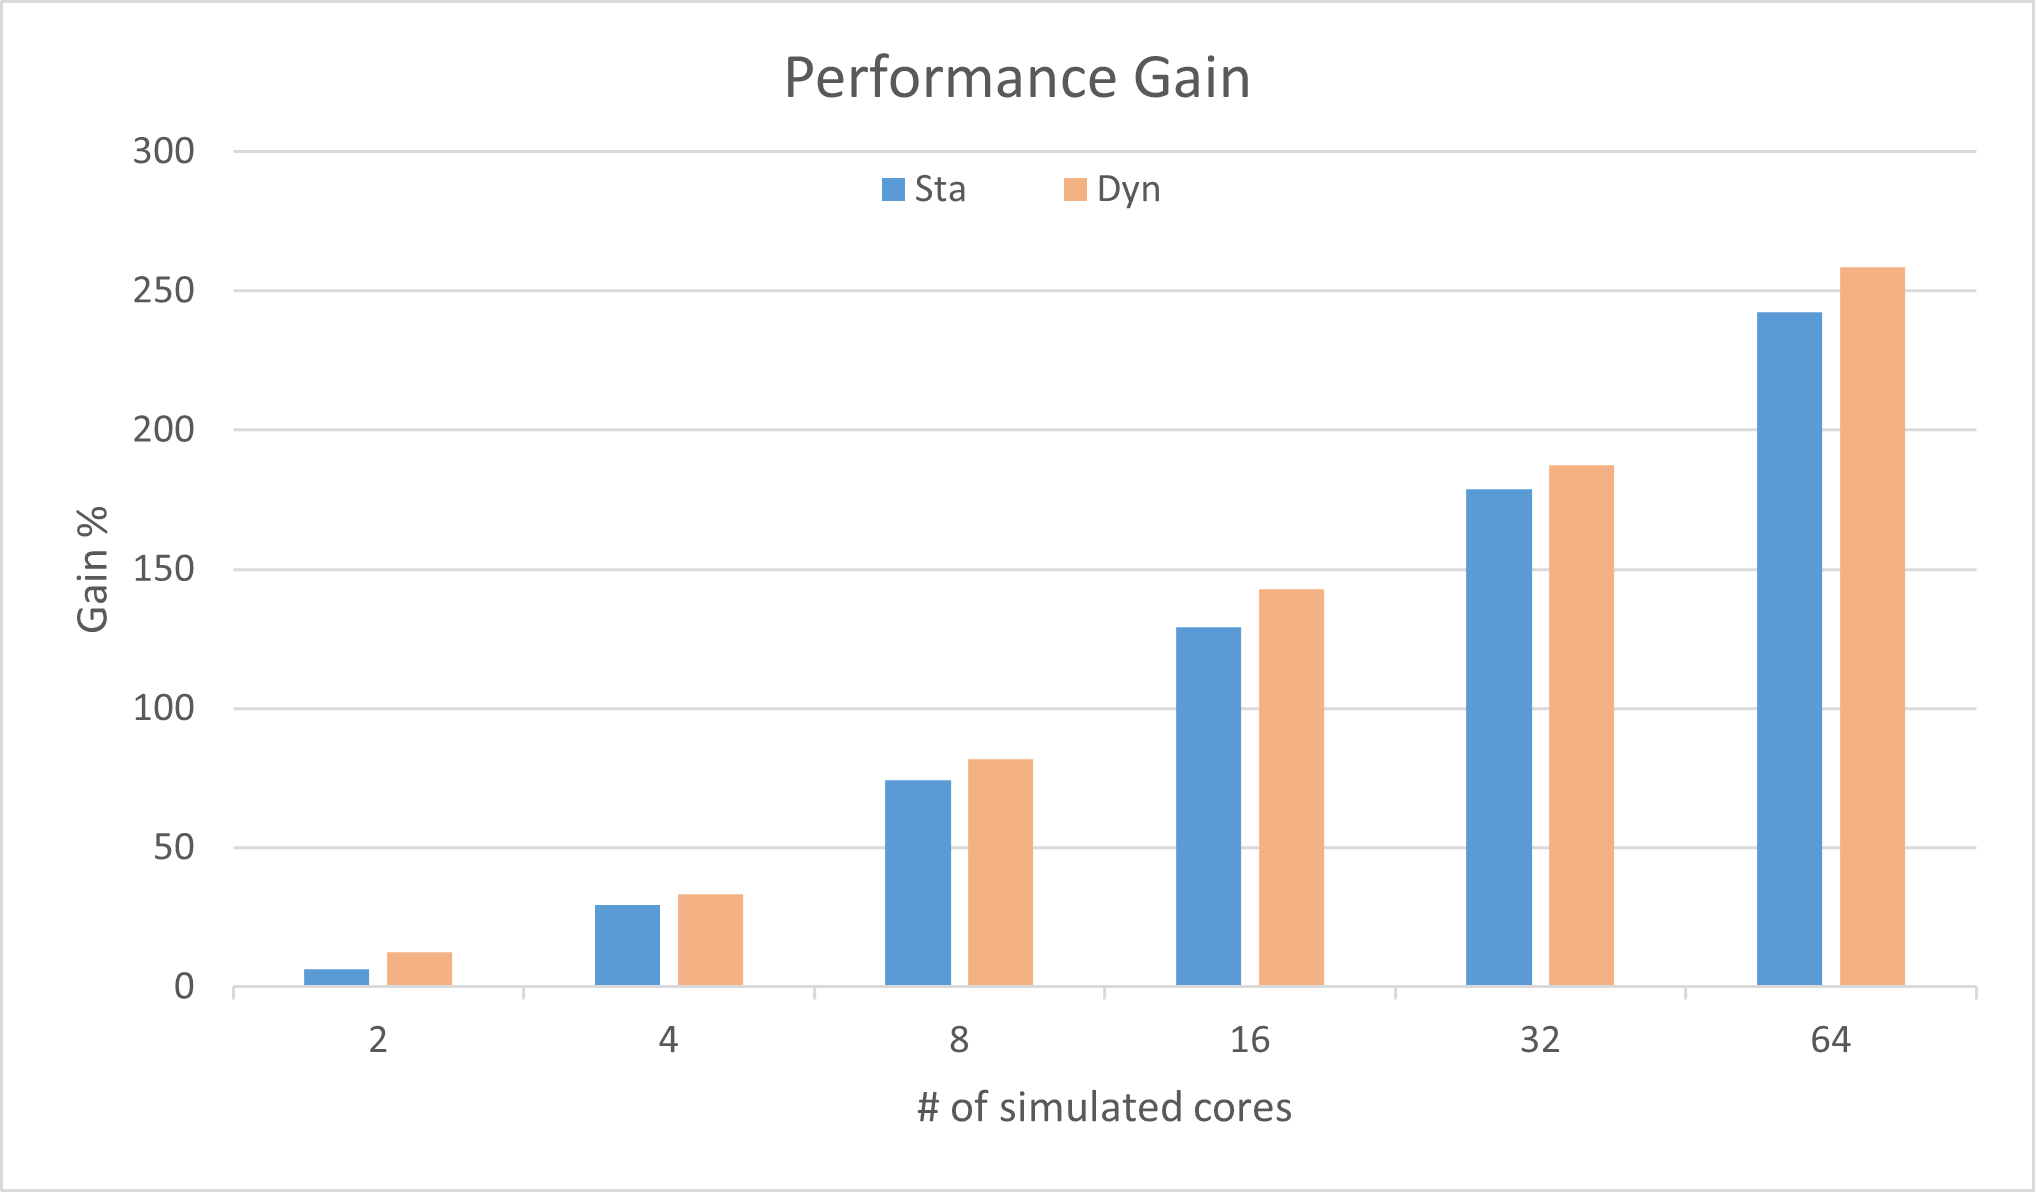
\includegraphics[width=0.75\textwidth]{Images/Performance_CO_SIM.png}
		\caption{ Performance gain}
		%\label{fig:Performance_ADA}
	\end{subfigure}
	\begin{subfigure}{\textwidth}
		\centering
		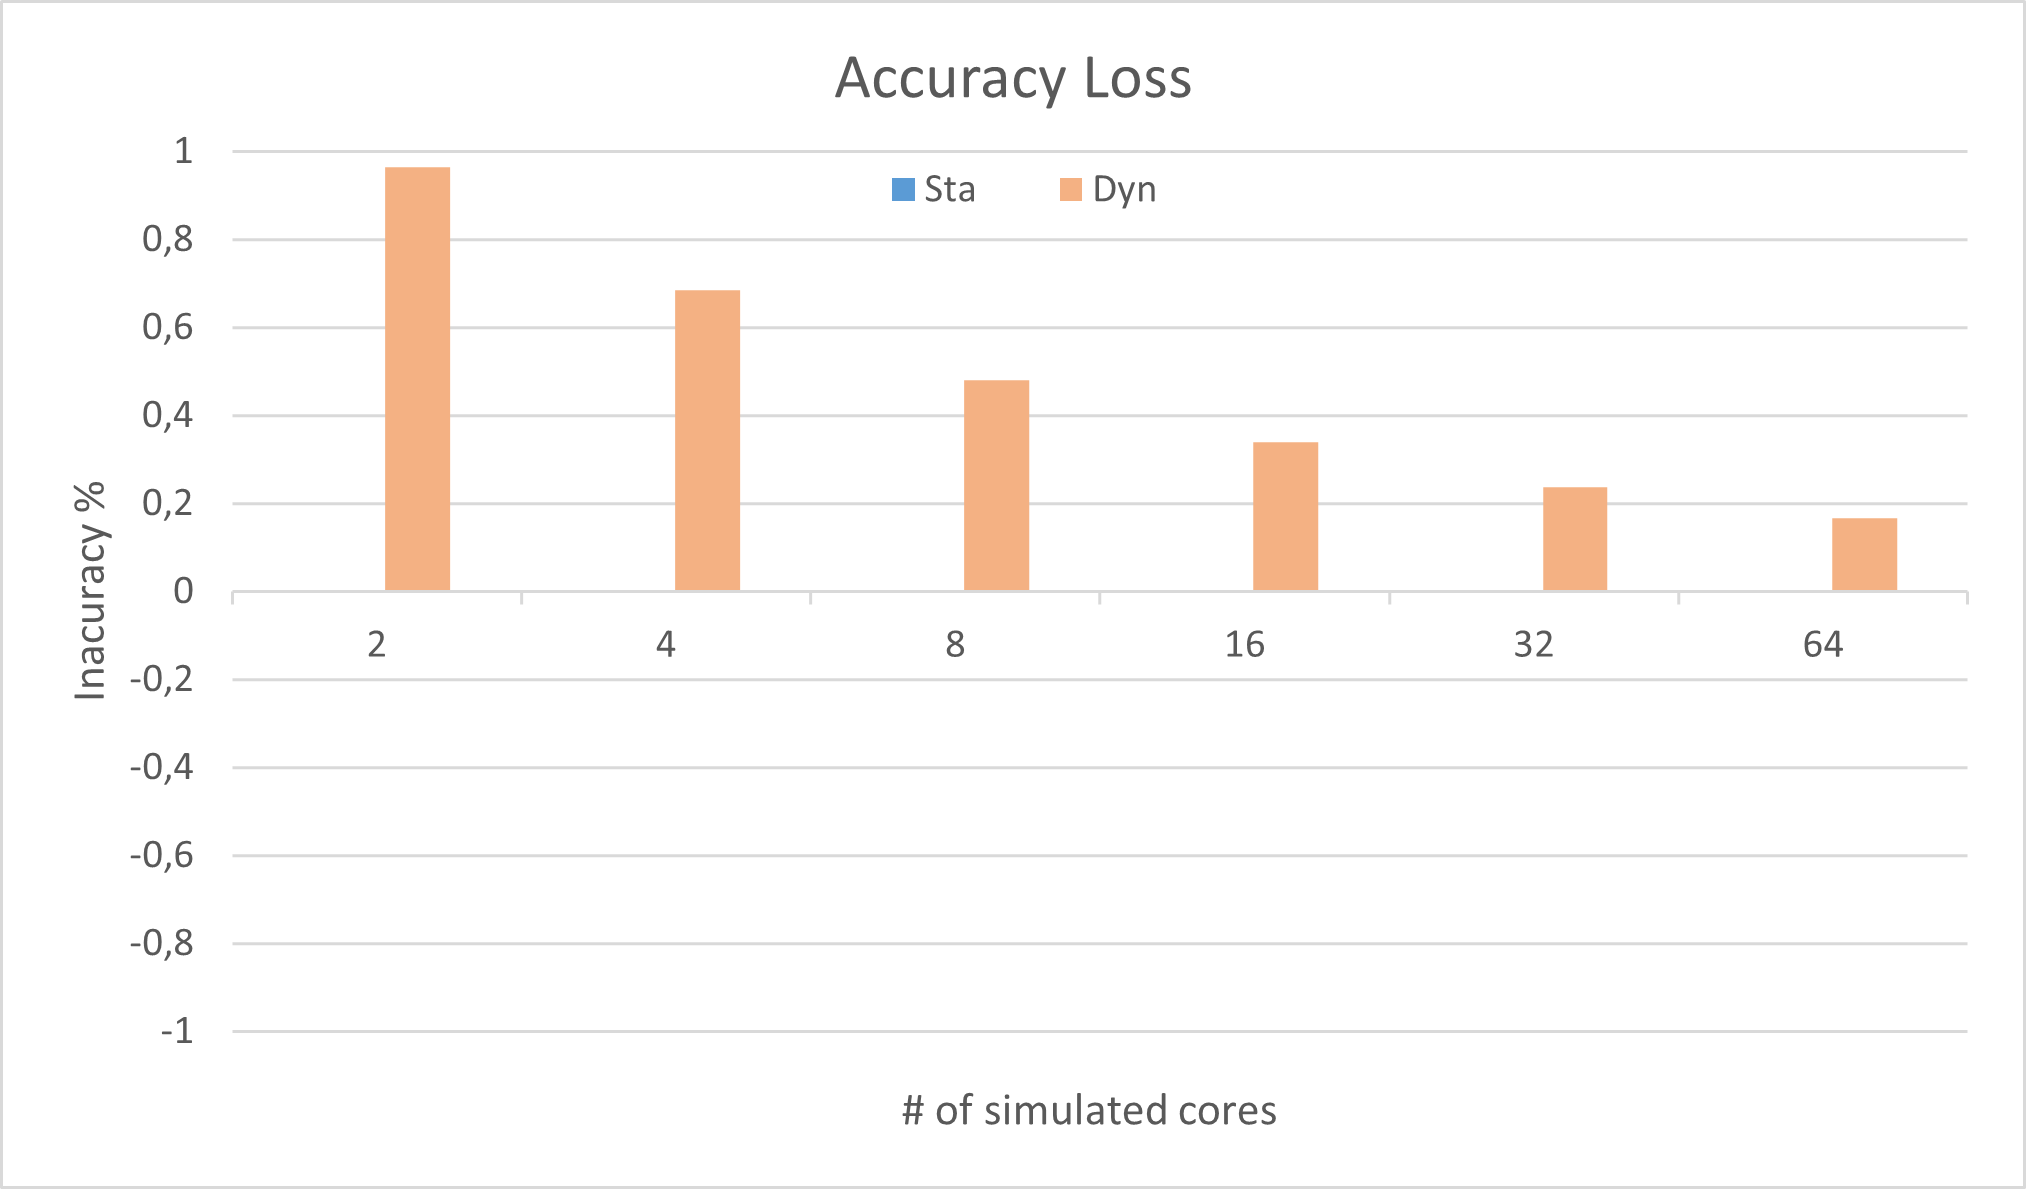
\includegraphics[width=0.75\textwidth]{Images/Accuracy_CO_SIM.png}
		\caption{ Accuracy lost}
		%\label{fig:Accuracy_ADA}
	\end{subfigure}
	\begin{subfigure}{\textwidth}
		\centering
		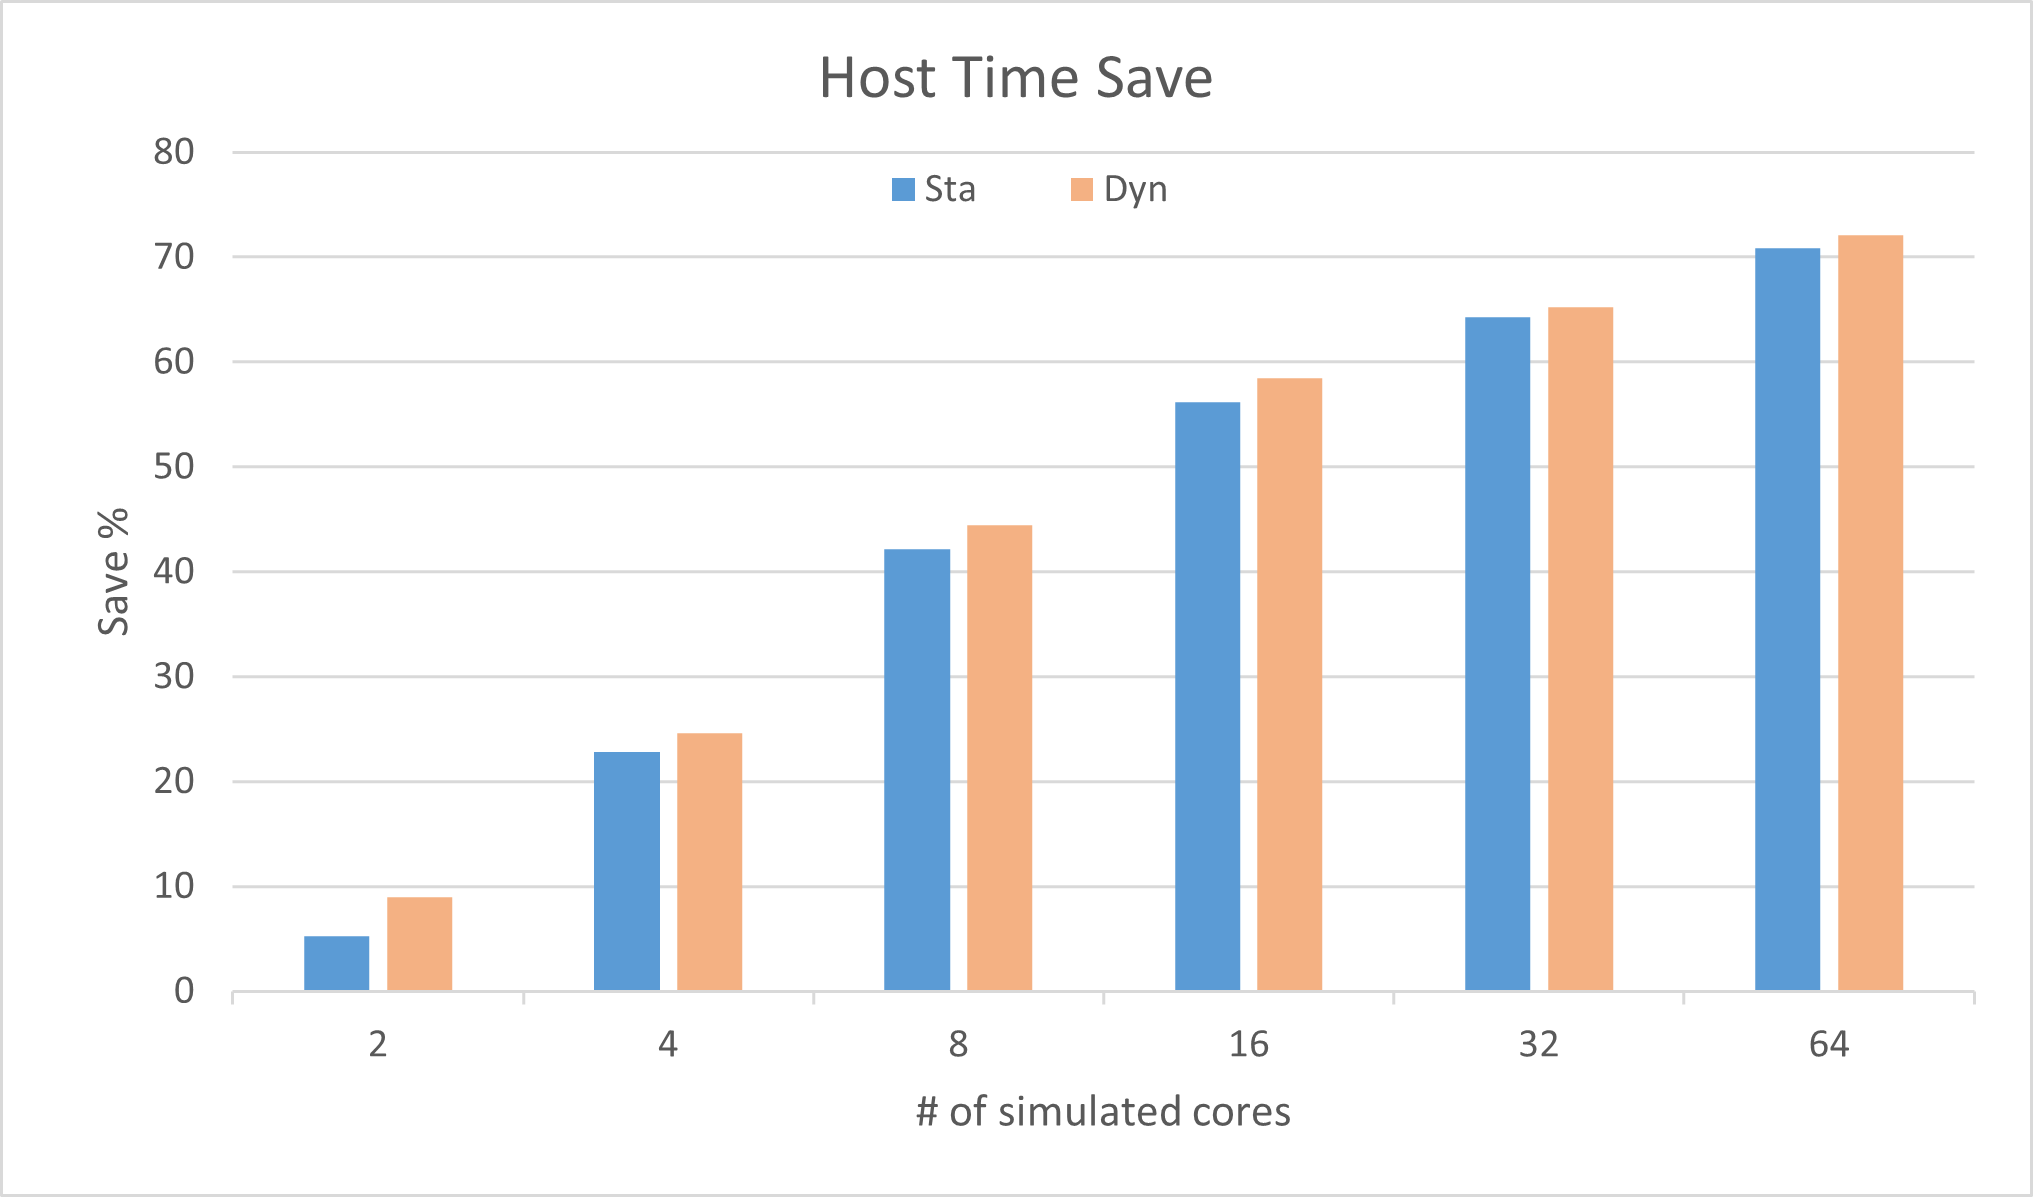
\includegraphics[width=0.75\textwidth]{Images/Host_CO_SIM.png}
		\caption{ Host time save}
		%\label{fig:Host_ADA}
	\end{subfigure}
			
	\caption{Co-simulation results}
	%\label{fig:results_ADA}
\end{figure}


The graphs illustrate the gains in comparison to the sequential simulation. Observing the images can be settled that the parallel version, either 
with the static or dynamic version had a better performance. With 64 simulated cores, the gains of the dynamic version overpassed 250\%. 
In fact, it can be affirmed that the performance gains grow with the increasing number of cores, due to the rise of workload amount. 
In terms of accuracy, the static version had almost a perfect result, while the dynamic one had 
a maximum inaccuracy of 0,98\% nevertheless, it is considerably far from the 5\%. Finally, as a consequence of the previously mentioned gains,
the host time was reduced, getting, in the majority of the cases, at least a reduction of 40\%. 


From these benchmarks other conclusions can be taken. Depending on the benchmark, the better simulation mode can differ from the sequential and
the parallel ones. It was verified that when the parallel tasks have considerable time consumption, the parallel mode gives more advantages 
since it can accelerate these, keeping the inaccuracy below 5\%. On the opposite way, if the communication between tools is where the simulation 
spends most of the time, the sequential mode will fit better, as it has a greater tradeoff between accuracy and performance. Further, the delay
times between the tasks also play a significant role. In cases where $T_{CoSim} >>> T_{ParTask}$, the parallel version is the most appropriate
otherwise, the sequential one should be chosen. 

In the end, to decide which mode is better for a certain workload, apriori information is needed.
If it does not exist, either because there is no documentation or the access to the source code is restricted, the better simulation mode to use, 
based on this case study, is the parallel mode with a dynamic quantum. The reason is that it had always an inaccuracy below 5\% and 
had a higher performance gain when compared to the sequential version. Nevertheless, if perfect accuracy is the main requirement, the 
sequential simulation mode should always be chosen.




